\documentclass[12pt]{fphw}

\usepackage[utf8]{inputenc}
\usepackage[T1]{fontenc}
\usepackage{mathpazo}
\usepackage{alphabeta}
\usepackage{graphicx}
\usepackage{booktabs}
\usepackage{listings}
\usepackage{enumerate}
\usepackage{hyperref}
\usepackage{amsmath}
\usepackage{framed}
\usepackage[framed]{ntheorem}
\usepackage{amssymb}
\usepackage{xcolor}
\usepackage{tabularx}
\usepackage{tikz}
\usepackage{float}
\usepackage{array}

\graphicspath{{./figures/}}

\setlength{\parskip}{\baselineskip}

\newframedtheorem{frm-thm}{Theorem}
\hypersetup{
    colorlinks=true,
    linkcolor=blue,
    filecolor=magenta,
    urlcolor=cyan,
}
\urlstyle{same}

\title{Deep Learning for NLP -- Homework 3 \\ Response Clarity Classification με Prompting Techniques (CLARITY)}
\author{Αλέξανδρος Γκιάφης \\ ID: sdi2200284 \\ Kaggle: \texttt{AlexTuring - sdi2200284}}
\date{Spring Semester 2025-2026}
\institute{National and Kapodistrian University of Athens \\ Department of Informatics and Telecommunications}
\class{Artificial Intelligence II (YS19 Μ226 Μ262 Μ325 Μ405)}

\begin{document}
\maketitle

{
  \hypersetup{linkcolor=black}
  \tableofcontents
}
\newpage

\section{Abstract}

Σε αυτή την τρίτη εργασία για το ίδιο dataset (CLARITY -- ταξινόμηση απαντήσεων πολιτικών σε \emph{Clear Reply}, \emph{Ambivalent}, \emph{Clear Non-Reply}) το paradigm άλλαξε εντελώς. Στην HW1 είχαμε φτιάξει vector-based classifiers (TF-IDF + Logistic Regression κ.λπ.). Στην HW2 κάναμε fine-tuning σε pretrained encoder Transformers (BERT, DistilBERT, DeBERTa). Εδώ στην HW3 δεν επιτρέπεται training καθόλου: παίρνουμε frozen instruction-tuned LLMs (\texttt{Qwen3.5-0.8B / 2B / 4B}) και τα ``πείθουμε'' με prompts να κάνουν τη δουλειά μας. Inference only.

Η εργασία ζητάει συστηματική σύγκριση τριών prompting στρατηγικών (\textbf{zero-shot}, \textbf{few-shot}, \textbf{chain-of-thought}) πάνω και στα τρία μεγέθη μοντέλου, δηλαδή ένα 3×3 grid, συν ότι άλλο prompting trick κρίνουμε χρήσιμο. Επίσης ζητάει subgroup analysis, error analysis, σύγκριση με τις προηγούμενες εργασίες, και την παράδοση \emph{ενός} Kaggle notebook με την πλήρη ανάλυση και το final submission.

\textbf{Το final σύστημά μου είναι \texttt{Qwen3.5-4B} + Chain-of-Thought prompt (το λέω \texttt{cot\_v4} στο report)}, με greedy decoding και χωρίς thinking mode. Στο τοπικό dev subset (500 stratified examples) πέτυχε macro-F1 \textbf{0.548}, στο test set (308 examples, με gold labels διαθέσιμα τοπικά από το HuggingFace) πέτυχε macro-F1 \textbf{0.575} και weighted-F1 \textbf{0.672}. Στο public Kaggle leaderboard (το οποίο χρησιμοποιεί weighted-F1 ως μετρική) έπιασε \textbf{0.72500}, που με βάλει σήμερα \textbf{3η θέση} (στο peak ήμουν 2ος). Σε σύγκριση με την HW2 όπου το DeBERTa fine-tuned είχε φτάσει 0.70 Kaggle, το prompting με ένα frozen 4B μοντέλο φτάνει \emph{γρηγορότερα} και πιο καθαρά, χωρίς να αγγίξουμε καθόλου weights.

Στις επόμενες ~30 σελίδες θα προσπαθήσω να αφηγηθώ ολόκληρη την πορεία της εργασίας με όσο πιο εκπαιδευτικό τρόπο μπορώ. Όπως και στην HW2, έχω βάλει συνειδητή προσπάθεια να εξηγώ \emph{και} τα βασικά concepts -- τι είναι ένα LLM, τι είναι ένα instruction-tuned μοντέλο, τι είναι η chain-of-thought reasoning, γιατί δουλεύει το prompting, γιατί τα chat templates -- χωρίς να τα θεωρώ self-evident. Όταν ξεκίνησα την εργασία αρκετά από αυτά τα ήξερα μόνο επιφανειακά, και θα ήθελα να τα είχα διαβάσει κάπου με αυτή τη λογική. Θα μιλήσω για ό,τι δοκίμασα, τι δούλεψε, τι όχι, και γιατί νομίζω.

\section{Εισαγωγή -- τι ακριβώς ζητάει η εκφώνηση}

\subsection{Το CLARITY task σε δύο λόγια}

Όπως ξέρω καλά πια από τις δύο προηγούμενες εργασίες, το CLARITY είναι ένα dataset από συνεντεύξεις και press conferences πολιτικών (κυρίως αμερικανών προέδρων -- Bush, Obama κ.λπ.) όπου το κάθε ζευγάρι \texttt{(question, answer)} έχει ένα label από τρία:

\begin{itemize}
    \item \textbf{Clear Reply} -- ο πολιτικός όντως απαντάει στο συγκεκριμένο πράγμα που ζητήθηκε. Πχ ``Q: \emph{What more can be done?} A: \emph{We've put a lot into ethanol\dots}''
    \item \textbf{Clear Non-Reply} -- ο πολιτικός ξεγλιστράει εντελώς. Δεν ασχολείται καν με το θέμα. Πχ ``Q: \emph{Have you seen any success?} A: \emph{I don't like talking about whether I see success or not\dots}''
    \item \textbf{Ambivalent} -- η μεγάλη γκρίζα ζώνη: λέει \emph{κάτι} σχετικό αλλά δεν δίνει στ' αλήθεια αυτό που του ζητήθηκε. Hedging, γενικότητες, μερικές απαντήσεις, talking around. Είναι περίπου το 59\% του dataset, οπότε αν ένα μοντέλο πει συνέχεια ``Ambivalent'' παίρνει accuracy 0.59 αλλά macro-F1 ~0.25.
\end{itemize}

Το task απαιτεί \emph{discourse-level reasoning} -- δεν αρκεί lexical overlap ή keyword matching. Πρέπει το μοντέλο να καταλάβει τη \emph{στάση} της απάντησης απέναντι στην ερώτηση, που είναι ένα πιο λεπτό σήμα από συχνότητες λέξεων. Στην HW1 αυτό ήταν ο βασικός λόγος που το TF-IDF κολλούσε γύρω στο 0.60. Στην HW2 το fine-tuned DeBERTa έφτασε ~0.70 χάρη σε contextual embeddings. Εδώ στην HW3 ψάχνουμε αν μπορεί το prompting σε ένα γενικό LLM να ανταγωνιστεί ή να ξεπεράσει.

\subsection{Τι αλλάζει η εκφώνηση σε σχέση με την HW2}

\begin{enumerate}
    \item \textbf{No training, only inference.} Δεν επιτρέπεται να ενημερώσουμε weights. Παίρνουμε frozen μοντέλα και τα ``ρωτάμε'' με prompts. Αυτό είναι ένα τελείως διαφορετικό paradigm από το fine-tuning.
    \item \textbf{Required μοντέλα: \texttt{Qwen3.5-0.8B}, \texttt{Qwen3.5-2B}, \texttt{Qwen3.5-4B}}. Αυτό μου το επιβεβαίωσε και ο instructor στο forum: είναι instruction-tuned LLMs με 3 διαφορετικά μεγέθη ώστε να φαίνεται καθαρά η επίδραση του size.
    \item \textbf{Required strategies: zero-shot, few-shot, chain-of-thought (CoT)}, και ότι άλλο prompting trick θεωρούμε σχετικό (self-consistency, role prompting, decomposition, κ.λπ.).
    \item \textbf{Ένα Kaggle notebook} με ολόκληρη την ανάλυση και το final submission (όχι τρία ξεχωριστά όπως στην HW2).
    \item \textbf{Random seed για reproducibility}. Στο prompting δεν υπάρχει random init του head όπως στο fine-tuning, αλλά το seed επηρεάζει τη subset επιλογή (αν δεν τρέχουμε σε όλα τα δεδομένα), την επιλογή few-shot examples, και -- αν χρησιμοποιήσουμε sampled decoding -- τις διαφορετικές γενιές.
    \item \textbf{Kaggle μετρική: F1-score}, και macro-F1 reported additionally. Στο report ζητάει accuracy, precision, recall, F1, macro-F1. Όπως αποδείχθηκε εκ των υστέρων, η Kaggle public leaderboard μετρική είναι το \emph{weighted}-F1, όχι το macro-F1 (αυτό φάνηκε από την υπεροχή του 0.725 LB σε σχέση με το 0.575 macro-F1 του τοπικού test).
    \item \textbf{Subgroup analysis ανά μήκος ερώτησης και μήκος απάντησης}, καθώς και \textbf{σύγκριση με HW1 και HW2}.
\end{enumerate}

\subsection{Το Kaggle notebook και το leaderboard result}

Το παραδοτέο Kaggle notebook είναι το \texttt{[sdi2200284] homework-3-prompting} (το έχω ονομάσει εσωτερικά \texttt{hw3-final}). Είναι διαμοιρασμένο με τη ΤΑ (\texttt{myrtotsokanaridou}) και δεν είναι public.

\textbf{Username στο Kaggle:} \texttt{AlexTuring - sdi2200284}.

\textbf{Public leaderboard score:} \textbf{0.72500} (weighted-F1). Αυτό σήμερα είναι η \textbf{3η θέση} στο public leaderboard, αφού δύο submissions πέρασαν μπροστά από το δικό μου την τελευταία στιγμή (ήμουν 2ος για αρκετές μέρες). Στο discord η συντριπτική πλειοψηφία των συμφοιτητών είχε scores ~0.27-0.42, και πιστεύω ότι το 0.725 ξεχωρίζει αρκετά καθαρά από αυτή την περιοχή.

Πρέπει επίσης να σημειώσω ότι το macro-F1 (η ``δίκαιη'' μετρική σε imbalanced setting) είναι σαφώς πιο χαμηλό από το weighted-F1 (0.575 vs 0.672 στο τοπικό test). Αυτό είναι αναμενόμενο και θα το συζητήσω: το weighted-F1 βαρύνει με το support, οπότε η μεγάλη Ambivalent class κυριαρχεί. Το macro-F1 δίνει ίσο βάρος στις 3 κλάσεις, οπότε η αποτυχία μου να πιάσω καθαρά την μειοψηφική Clear Non-Reply (CNR F1 ~0.39) φαίνεται περισσότερο.

\subsection{Γιατί αυτή η εργασία είναι ποιοτικά διαφορετική}

Στην HW2 έπρεπε να γράψω custom PyTorch training loop, να ασχοληθώ με optimizer, learning rates, schedulers, gradient clipping, mixed precision -- δηλαδή \emph{πώς} εκπαιδεύεται ένα μοντέλο. Εδώ τίποτα από όλα αυτά. Το μοντέλο είναι έτοιμο. Το ζήτημα είναι \emph{πώς το ρωτάς}.

Αυτή η μετατόπιση είναι θεμελιώδης. Στο fine-tuning, οι ``hyperparameters'' είναι learning rate, batch size, epochs, decay. Στο prompting, τα ισοδύναμα είναι:

\begin{itemize}
    \item το \emph{prompt} (text) -- system prompt, instructions, formatting, label specification
    \item τα \emph{decoding settings} -- greedy vs sampling, temperature, top-p, top-k, max\_new\_tokens
    \item το αν δίνουμε few-shot examples και ποια
    \item το αν ζητάμε reasoning (CoT) και πώς
    \item το \emph{output parsing} -- πώς εξάγουμε το final label από το text που γενιάει το μοντέλο
\end{itemize}

Όλα αυτά είναι μη-διαφορίσιμα knobs, χωρίς gradient descent. Η ``εκπαίδευση'' γίνεται στο μυαλό μου: τρέχω κάτι, βλέπω τι κάνει λάθος, σκέφτομαι γιατί, αλλάζω το prompt, ξανατρέχω. Είναι πιο κοντά σε ``software engineering of prompts'' παρά σε ``machine learning''. Και αυτό έχει πραγματικές συνέπειες σε αυτό που μπορεί να γίνει: στο fine-tuning, αν έχεις labelled data, σε ένα κλειστό task σαν αυτό, μπορείς να μάθεις labels που είναι αυθαίρετα. Στο prompting, αν το LLM δεν έχει ήδη κάποια idea για το concept ``Clear Reply vs Ambivalent vs Clear Non-Reply'', δύσκολα θα το διδάξεις με λίγα λόγια.

\section{Πριν προχωρήσω -- βασικές έννοιες για όποιον δεν τις ξέρει}

Όπως και στην HW2 report, βάζω εδώ μια ενότητα όπου εξηγώ τα concepts που χρησιμοποιώ. Είναι ο αναγνώστης που μόλις άκουσε για το ``LLM'' και θέλει να καταλάβει τι κάνει αυτή η εργασία, οπότε εξηγώ από την αρχή. Αν τα ξέρετε όλα, μπορείτε να προχωρήσετε.

\subsection{Τι είναι ένα Large Language Model}

Ένα \emph{Large Language Model} (LLM) είναι, στην απλούστερη του μορφή, μια συνάρτηση που παίρνει μια ακολουθία από tokens και μαντεύει το επόμενο. Δηλαδή αν του δώσεις ``The capital of France is'', θα προβλέψει με πολύ υψηλή πιθανότητα ότι το επόμενο token είναι ``Paris''.

Αυτή η συνάρτηση είναι ένα νευρωνικό δίκτυο τύπου Transformer \cite{vaswani2017attention} με τεράστιο αριθμό παραμέτρων (μερικά δισ.\ έως μερικά τρισ.). Εκπαιδεύεται σε τεράστια ποσότητα κειμένου (Wikipedia, books, internet) με ένα απλό task: για κάθε σημείο της ακολουθίας, να προβλέπει το επόμενο token. Αυτό λέγεται \emph{next-token prediction} ή \emph{causal language modeling}.

Επειδή ο όγκος των δεδομένων είναι τεράστιος και η αρχιτεκτονική έχει χωρητικότητα, το μοντέλο μαθαίνει πολύ πέρα από ``ποια λέξη ακολουθεί ποια''. Μαθαίνει σύνταξη, σημασιολογία, μερικές προγραμματιστικές γλώσσες, λίγη μαθηματική λογική, μια εκτενή γενική γνώση για τον κόσμο, ακόμα και reasoning patterns. Είναι ένα emergent behavior από το scale.

Η μαγική ιδιότητα των LLMs είναι το \emph{in-context learning}: ακόμα κι αν το μοντέλο δεν εκπαιδεύτηκε ποτέ στο συγκεκριμένο task μας, μπορεί να το ``καταλάβει'' απλώς διαβάζοντας μια περιγραφή του ή μερικά παραδείγματα στο prompt. Δεν αλλάζουν weights -- το μοντέλο, σε inference time, χρησιμοποιεί το context να καθοδηγήσει τη συμπεριφορά του.

\subsection{Decoder-only Transformer -- η αρχιτεκτονική των LLMs}

Το BERT/DeBERTa της HW2 ήταν \emph{encoder-only} Transformers. Έπαιρναν την πρόταση όλη μαζί, υπολόγιζαν bidirectional attention (κάθε λέξη βλέπει \emph{όλες}), και έβγαζαν αναπαραστάσεις χρήσιμες για ταξινόμηση. Δεν παρήγαγαν κείμενο.

Τα Qwen3.5 (όπως και GPT, LLaMA, Mistral, κ.λπ.) είναι \emph{decoder-only} Transformers. Είναι \emph{causal}: κάθε token βλέπει μόνο τα προηγούμενα tokens, όχι τα επόμενα. Αυτό γίνεται με ένα ``causal mask'' στην self-attention, που μηδενίζει τις θέσεις στο μέλλον. Έτσι το μοντέλο μαθαίνει να προβλέπει αυτό-που-είναι-μετά μόνο από αυτό-που-ήταν-πριν, που είναι ακριβώς αυτό που χρειάζεται για generation.

Στο inference, παράγουμε ένα token τη φορά: τρέχουμε ένα forward pass, παίρνουμε τα logits του τελευταίου token, διαλέγουμε το επόμενο, το προσθέτουμε στο context, ξανατρέχουμε. Επαναλαμβάνουμε μέχρι το μοντέλο να βγάλει ένα \texttt{EOS} (end-of-sequence) token ή να φτάσουμε στο όριο που έχουμε ορίσει (\texttt{max\_new\_tokens}).

\subsection{Pretraining vs Instruction tuning -- οι δύο φάσεις των LLMs}

Είναι κρίσιμο να ξεχωρίσουμε δύο φάσεις στην εκπαίδευση ενός σύγχρονου LLM:

\textbf{Φάση 1: Pretraining.} Το μοντέλο εκπαιδεύεται σε τρισεκατομμύρια tokens κειμένου με causal language modeling. Στο τέλος, ξέρει να συνεχίζει κείμενο αλλά \emph{δεν} ξέρει απαραίτητα να ακολουθεί οδηγίες. Αν του δώσεις ``Translate to French: hello'', μπορεί να σου απαντήσει ``bonjour'' ή να σου γράψει ένα διάλογο όπου κάποιος δίνει αυτή την οδηγία -- δεν ξεχωρίζει instruction από context.

\textbf{Φάση 2: Instruction tuning + RLHF.} Παίρνουμε το pretrained μοντέλο και το \emph{fine-tunάρουμε} σε ζεύγη \texttt{(instruction, ideal response)} \cite{wei2022instructiontuned,ouyang2022instructgpt}. Συνήθως αυτό γίνεται σε δύο μέρη:

\begin{itemize}
    \item \emph{Supervised fine-tuning (SFT)}: ανθρώπινα-γραμμένα ζεύγη instruction/απάντηση.
    \item \emph{Reinforcement Learning from Human Feedback (RLHF)}: το μοντέλο παράγει πολλές υποψήφιες απαντήσεις, άνθρωποι τις βαθμολογούν, και ένα reward model μαθαίνει την κατάταξη. Μετά κάνουμε RL (PPO ή DPO) έτσι ώστε το μοντέλο να παράγει απαντήσεις που το reward model θεωρεί καλύτερες.
\end{itemize}

Μετά από αυτό το pipeline, το μοντέλο έχει μάθει το ``chat assistant'' rôle: δίνεις οδηγία, σε απαντάει με τη μορφή που του ζήτησες. Όλα τα Qwen3.5-X-Instruct (που χρησιμοποιώ εδώ) είναι instruction-tuned.

Αυτή η διάκριση έχει σημασία για το prompting. Το instruction-tuned μοντέλο ``καταλαβαίνει'' γενικές οδηγίες όπως ``classify this answer into one of three categories''. Ένα base (μη instruction-tuned) μοντέλο πιθανότατα θα συνέχιζε το prompt μου αντί να εκτελέσει την οδηγία.

\subsection{Tokenization στα LLMs}

Όπως και στους encoders, οι LLMs δουλεύουν με subword tokens. Το Qwen χρησιμοποιεί \emph{Byte-Pair Encoding (BPE)} με vocabulary ~150k tokens. Ένα Greek κείμενο μπορεί να χρειαστεί 2-3× περισσότερα tokens από αντίστοιχο αγγλικό γιατί το BPE είναι κυρίως βελτιστοποιημένο για αγγλικά.

Αυτό είναι σημαντικό για budgeting. Σε ένα input \texttt{Question: \dots Answer: \dots} όπου η απάντηση είναι π.χ.\ 300 λέξεις, το input μπορεί να είναι ~450-500 tokens. Το system prompt (όπου περιγράφω το task) είναι ~250 tokens, τα CoT instructions ~80 tokens. Σύνολο prompt: 700-800 tokens. Το μοντέλο μετά παράγει 100-200 tokens reasoning. Συνολικό context: ~1000 tokens, κάτω από τα 32k που υποστηρίζει το Qwen3.5, οπότε δεν είχα ποτέ context-length issues.

\subsection{Chat template -- πώς ``μιλάμε'' με ένα chat model}

Όταν ένα μοντέλο γίνει instruction-tuned, εκπαιδεύεται σε ένα ειδικό format διαλόγου -- συνήθως ChatML ή κάτι παρόμοιο. Στο Qwen3.5 το format μοιάζει με:

\begin{verbatim}
<|im_start|>system
You are an expert annotator for political interviews...
<|im_end|>
<|im_start|>user
Question: ...
Answer: ...
<|im_end|>
<|im_start|>assistant
\end{verbatim}

Το μοντέλο περιμένει αυτές τις ακριβείς ``δομές'' (special tokens και role tags) γιατί έτσι το εκπαιδεύσαμε. Αν δίναμε raw text χωρίς αυτά, η ποιότητα θα έπεφτε δραματικά.

Στο HuggingFace, η Transformers library παρέχει τη μέθοδο \texttt{tokenizer.apply\_chat\_template(messages, add\_generation\_prompt=True)} που μου χτίζει το σωστό prompt format από μια λίστα μηνυμάτων ρόλου-περιεχομένου. Όλο το codebase μου περνάει από αυτή τη μέθοδο, ποτέ δεν χτίζω chat prompts στο χέρι.

\subsection{Decoding strategies -- πώς διαλέγουμε το επόμενο token}

Σε κάθε βήμα, το μοντέλο βγάζει logits πάνω από όλο το vocabulary (~150k τιμές). Με softmax τα κάνουμε probability distribution. Τι κάνουμε με αυτό;

\begin{itemize}
    \item \textbf{Greedy decoding}: \texttt{do\_sample=False}. Παίρνουμε το argmax (πιο πιθανό token σε κάθε βήμα). Deterministic, αναπαραγώγιμο, fast. Συνήθως σωστό σε classification-style tasks.
    \item \textbf{Sampling}: \texttt{do\_sample=True}, \texttt{temperature=T}. Δειγματοληψία από το distribution. Μεγαλύτερο T = πιο τυχαία, μικρότερο = πιο deterministic. Πιο δημιουργικό αλλά πιο noisy.
    \item \textbf{Top-k / top-p (nucleus) sampling}: περιορίζουμε το sampling στο top-k πιο πιθανά tokens, ή στο μικρότερο σύνολο tokens που μαζί έχουν probability ≥ p. Αποφεύγουμε ``ψυχωτικά'' tokens που έχουν πιθανότητα 1e-6.
\end{itemize}

Για το CLARITY task, το logical choice είναι \emph{greedy decoding}. Δεν θέλω creative παραγωγή, θέλω σταθερή ταξινόμηση. Όλα τα experimental runs μου χρησιμοποιούν \texttt{do\_sample=False}. Η μόνη εξαίρεση είναι το self-consistency πείραμα (Phase 5.5), όπου σκόπιμα χρησιμοποίησα sampling για να πάρω πολλαπλά reasoning paths και να ψηφίσω.

\subsection{Prompting -- η ``προγραμματιστική'' γλώσσα των LLMs}

\emph{Prompt} είναι το input text που δίνουμε στο μοντέλο. \emph{Prompting} είναι η τέχνη να γράφουμε prompts που οδηγούν το μοντέλο στη συμπεριφορά που θέλουμε. Σε ένα frozen μοντέλο, το prompt είναι το μόνο knob.

Το γενικό σχήμα ενός prompt σε classification task είναι:

\begin{verbatim}
[System role]   instructions: τι είσαι, τι κάνεις, τι labels δίνεις
[User turn]     το συγκεκριμένο input (question + answer)
[Assistant]     (το μοντέλο γενιάει εδώ το label)
\end{verbatim}

Το ``πώς γράφω το instructions'' είναι ολόκληρη επιστήμη που τη λένε \emph{prompt engineering}. Οι βασικές διαστάσεις είναι: ορισμοί κλάσεων, decision criteria, demonstration examples (few-shot), reasoning instructions (CoT), output format, edge case guidance.

\subsection{Zero-shot, few-shot, chain-of-thought}

Οι τρεις κύριες οικογένειες prompting strategies που ζητάει η εκφώνηση:

\textbf{Zero-shot}: λέμε στο μοντέλο τι να κάνει χωρίς να του δώσουμε παραδείγματα.

\begin{verbatim}
You are a classifier. Classify the answer into Clear Reply, Ambivalent,
or Clear Non-Reply.
Question: [Q]
Answer: [A]
Label:
\end{verbatim}

\textbf{Few-shot} \cite{brown2020gpt3}: του δίνουμε k παραδείγματα (input + correct label) στο prompt πριν από το ζητούμενο.

\begin{verbatim}
You are a classifier.
Example 1:
Question: [Q1] Answer: [A1] Label: Clear Reply
Example 2:
Question: [Q2] Answer: [A2] Label: Ambivalent
...
Now classify:
Question: [Q] Answer: [A] Label:
\end{verbatim}

Η ιδέα: το μοντέλο μαθαίνει το format και ίσως το decision boundary από τα examples (\emph{in-context learning}).

\textbf{Chain-of-Thought (CoT)} \cite{wei2022cot}: αντί να ζητάμε από το μοντέλο να απαντήσει αμέσως, του ζητάμε να ``σκεφτεί βήμα-βήμα'' πριν δώσει το final answer.

\begin{verbatim}
Think step by step:
1. What does the question ask for?
2. What does the answer provide?
3. Does the answer give that specific information?
Then write: Label: <one of the three>
\end{verbatim}

Η αρχική παρατήρηση των Wei et al.\ 2022 ήταν ότι σε arithmetic / reasoning tasks, το CoT δίνει μεγάλα gains -- κάποια αδιόρθωτα tasks ξαφνικά λύνονται. Η intuition είναι ότι το LLM ``σκέφτεται φωναχτά'' και αυτό του δίνει επιπλέον υπολογιστικό χώρο πριν δεσμευτεί σε απάντηση.

Δεν είναι σαφές αν αυτό βοηθάει στο CLARITY task -- δεν είναι αυστηρά μαθηματικό. Αλλά αποδείχθηκε ότι βοηθάει τεράστια, και αυτό είναι από τα πιο ενδιαφέροντα findings της εργασίας.

\subsection{Self-consistency}

Μια επέκταση του CoT \cite{wang2023selfconsistency}: αντί για ένα reasoning path, παράγουμε K διαφορετικά (με sampling) και ψηφίζουμε στο final label (\emph{majority vote}). Η intuition: αν το μοντέλο φτάνει στο ίδιο label από πολλαπλά reasoning paths, μάλλον είναι σωστό. Αν αλλάζει, μάλλον είναι αβέβαιο.

Όπως θα δω σε λίγο, στο δικό μου task το SC δεν δούλεψε. Θα συζητήσω γιατί.

\subsection{Evaluation metrics για classification (γρήγορη αναφορά)}

Επειδή έχω εξηγήσει αυτά αναλυτικά στην HW2 report, εδώ κάνω μόνο μια γρήγορη αναφορά:

\begin{itemize}
    \item \textbf{Accuracy}: $\frac{\text{σωστές}}{\text{σύνολο}}$. Παραπλανητικό σε imbalanced data.
    \item \textbf{Precision (ανά κλάση)}: $\frac{TP}{TP+FP}$ -- πόσο σωστές είναι οι θετικές προβλέψεις του μοντέλου.
    \item \textbf{Recall (ανά κλάση)}: $\frac{TP}{TP+FN}$ -- πόσα από τα πραγματικά positives πιάνει το μοντέλο.
    \item \textbf{F1 (ανά κλάση)}: harmonic mean των precision και recall.
    \item \textbf{Macro-F1}: μέσος όρος των F1 ανά κλάση. Ίσο βάρος στις 3 κλάσεις. \textbf{Η δίκαιη μετρική σε imbalanced settings.}
    \item \textbf{Weighted-F1}: $\sum_c \text{support}_c \cdot F_{1,c} / N$. Δίνει έμφαση στην πλειονοτική κλάση. \textbf{Είναι αυτή που χρησιμοποιεί το Kaggle.}
    \item \textbf{Invalid rate}: το ποσοστό των μοντέλο-γενιών που δεν παρσάρονται σε valid label. Αν > 0\%, το post-processing είναι buggy ή το μοντέλο αρνείται να ακολουθήσει το format.
\end{itemize}

Για το CLARITY, το ``δίκαιο'' macro-F1 είναι αυτό που χρησιμοποιώ στο report ως κύρια μετρική (όπως ζητάει η εκφώνηση), αλλά αναφέρω και το weighted-F1 γιατί αυτό μετράει στο Kaggle.

\subsection{Mini-glossary}

\begin{itemize}
    \item \textbf{Token}: η μονάδα στην οποία δουλεύει το μοντέλο. Όχι ακριβώς λέξη, ούτε character -- κάτι ενδιάμεσο (subword).
    \item \textbf{Context length}: το μέγιστο πλήθος tokens που μπορεί να ``δει'' το μοντέλο σε ένα call. Για το Qwen3.5 είναι 32k.
    \item \textbf{max\_new\_tokens}: το μέγιστο πλήθος tokens που θα παράγει στην απάντηση.
    \item \textbf{Logits}: πριν το softmax. Output του μοντέλου σε raw αριθμούς.
    \item \textbf{System prompt / user message / assistant message}: τα τρία ρόλους ενός chat conversation.
    \item \textbf{Greedy / sampled decoding}: deterministic argmax vs probabilistic sampling για κάθε token.
    \item \textbf{In-context learning}: η ικανότητα του μοντέλου να ``καταλάβει'' το task από το prompt χωρίς weight updates.
    \item \textbf{Thinking mode (Qwen-specific)}: το Qwen3 έχει ένα ειδικό mode όπου παράγει ένα εκτενές thinking trace μέσα σε \texttt{<think>\dots</think>} tags πριν δώσει την τελική απάντηση. Όταν είναι ενεργό μπορεί να καίει χιλιάδες output tokens. Στη δουλειά μου έχω \texttt{enable\_thinking=False} -- αρκεί η δική μου explicit CoT instruction.
    \item \textbf{bf16}: 16-bit brain float -- το format που τρέχει το μοντέλο για να χωράει σε GPU memory. Μικρό numerical noise vs fp32 αλλά κανονικά δεν μεταβάλλει τα αποτελέσματα ποιοτικά.
\end{itemize}

OK, νομίζω αυτά είναι αρκετά για βάσεις. Πάμε στα μοντέλα.

\section{Τα τρία μοντέλα -- αναλυτικός οδηγός}

Η εκφώνηση καθορίζει τα τρία μοντέλα: \texttt{Qwen/Qwen3.5-0.8B}, \texttt{Qwen/Qwen3.5-2B}, \texttt{Qwen/Qwen3.5-4B}. Όλα ανήκουν στην οικογένεια \textbf{Qwen3.5} της \emph{Alibaba}, και είναι όλα instruction-tuned variants.

\subsection{Qwen3.5 -- η οικογένεια}

Το Qwen \cite{qwen3technical} είναι μια οικογένεια ανοιχτών LLMs από την Alibaba, με τρέχουσα γενιά την Qwen3 (Spring 2025). Η Qwen3.5 είναι μια ενδιάμεση revision που έβγαλε στις αρχές του 2026 (μεγαλύτερο pretraining corpus, ενημερωμένο instruction tuning).

Τα μεγέθη που χρησιμοποιώ: 0.8B, 2B, 4B παράμετροι. Όλα δίνονται και ως base και ως instruction-tuned. Εδώ χρησιμοποιώ τις instruction-tuned εκδόσεις (ονόματα HF \texttt{Qwen/Qwen3.5-X}, που είναι already instruction-tuned σε αυτή τη γενιά -- δεν χρειάζεται explicit \texttt{-Instruct} suffix). Είναι decoder-only Transformers, παρόμοιες με LLaMA-style architecture (RMSNorm, SwiGLU activation, Rotary Positional Embeddings, Grouped-Query Attention).

\textbf{Πέντε χαρακτηριστικά της οικογένειας Qwen3 που είναι χρήσιμα να ξέρει κανείς}:

\begin{enumerate}
    \item \textbf{Instruction-tuned by default}: αυτά τα names HF βγάζουν instruction-tuned models -- δεν χρειάζεται separate fine-tuning.
    \item \textbf{32k context length}: άνετα χωράει τα δικά μου prompts.
    \item \textbf{Multilingual}: το pretraining corpus περιλαμβάνει >100 γλώσσες, οπότε ξέρει αρκετά καλά Greek, αλλά τα prompts μου είναι όλα αγγλικά γιατί το CLARITY είναι αγγλόφωνο.
    \item \textbf{Thinking mode}: στις πιο πρόσφατες εκδόσεις, μπορείς να ζητήσεις από το μοντέλο να ``σκεφτεί'' σε ξεχωριστή ενότητα (\texttt{<think>\dots</think>}) πριν απαντήσει. Στη δουλειά μου το έχω σβηστό (\texttt{enable\_thinking=False}) γιατί ήδη ζητάω explicit CoT μέσα στο user prompt, και το thinking mode μπορεί να καίει χιλιάδες tokens.
    \item \textbf{Chat template}: ChatML-like format με \texttt{<|im\_start|>}, \texttt{<|im\_end|>}. Το HF tokenizer το χειρίζεται μόνο του.
\end{enumerate}

\subsection{Qwen3.5-0.8B}

Το ``μικρό'' της οικογένειας. 0.8 δισ.\ παράμετροι. Πολύ γρήγορο -- σε Kaggle T4 (16GB) τρέχει ~10× ταχύτερα από το 4B στο ίδιο prompt.

\textbf{Πότε το χρησιμοποιώ}: για \emph{όλο} το prompt iteration. Δοκιμάζω 4-5 prompt variants σε ένα dev subset, βλέπω ποιο δίνει νόημα, και προωθώ στα μεγαλύτερα μοντέλα μόνο όσα κρίνω αξιόλογα. Με αυτή τη στρατηγική (``screen on small, confirm on large'') εξοικονόμησα τεράστιες GPU ώρες.

\textbf{Όρια του 0.8B σε αυτό το task}: είναι αρκετά ``naive''. Στο zero-shot με naive prompt καταρρέει σε μία μόνο κλάση (όλα Clear Non-Reply). Χρειάζεται explicit ορισμούς και rubric να φτάσει στο 0.30 macro-F1. Με CoT φτάνει 0.42. Δεν μπορεί όμως ποτέ να πιάσει το 4B+CoT (0.55). Το reasoning capacity είναι περιορισμένο.

\subsection{Qwen3.5-2B}

Το ``μεσαίο''. 2 δισ.\ παράμετροι. Καλή ισορροπία ταχύτητας και ποιότητας. Στο Kaggle T4 τρέχει ~3-4× πιο γρήγορα από το 4B.

\textbf{Στο grid μου}: zero-shot 0.393, few-shot 0.381, CoT 0.488. Αξιόλογη βελτίωση σε σχέση με το 0.8B, και το CoT συνεχίζει να είναι το καλύτερο.

\subsection{Qwen3.5-4B}

Το ``μεγάλο'' (το μεγαλύτερο που μπορώ να τρέξω σε Kaggle T4 με bf16). 4 δισ.\ παράμετροι. Είναι αυτό που τελικά δίνει το best score της εργασίας.

\textbf{Στο grid μου}: zero-shot \emph{0.318 -- collapse}, few-shot 0.414, CoT \textbf{0.548 (best)}. Το zero-shot collapse είναι από τα πιο ενδιαφέροντα findings: το μεγαλύτερο μοντέλο, \emph{χειρότερο} από το μεσαίο όταν χρησιμοποιεί zero-shot. Θα το αναλύσω παρακάτω.

\subsection{Γιατί δεν δοκίμασα ακόμα μεγαλύτερα μοντέλα}

Η εκφώνηση επιτρέπει να δοκιμάσω και άλλες model families ή μεγέθη, αλλά:

\begin{itemize}
    \item Το 7B / 8B Qwen δεν χωράει σε Kaggle T4 (16GB VRAM) σε bf16 χωρίς aggressive quantization. Με 4-bit quantization θα έχανα ποιότητα και δεν θα ήταν fair η σύγκριση.
    \item Δεν είχα πρόσβαση σε Colab Pro / άλλο GPU σε αυτή τη φάση του εξαμήνου, οπότε ο compute budget μου ήταν Kaggle's 30h/week.
    \item Η εκφώνηση είπε ρητά ``Qwen comparison is the core requirement''. Επομένως 0.8B / 2B / 4B καλύπτουν το ζητούμενο spectrum.
\end{itemize}

\subsection{Τα όρια των μικρών LLMs σε αυτό το task}

Πριν μπω στα πειράματα, μια γενική παρατήρηση που νομίζω αξίζει να γίνει εξαρχής: \textbf{το CLARITY είναι ένα δύσκολο task για μικρά μοντέλα}. Το hardest class (Clear Non-Reply) είναι μειοψηφικό, και η διάκριση Ambivalent vs Clear Reply απαιτεί λεπτή discourse-level κρίση που δεν είναι μέρος του standard pretraining mix.

Στη βιβλιογραφία, prompting με 7B-13B μοντέλα φτάνει χαμηλό macro-F1 σε άλλα subjective classification tasks (sentiment subtleties, sarcasm detection, irony). Με 0.8B-4B εδώ, ένα macro-F1 0.55 είναι όντως καλό. Το ταβάνι του prompted approach σε αυτό το task μάλλον είναι κάπου στο 0.65-0.70 με πολύ μεγαλύτερα μοντέλα και πιο εκτενή prompting techniques (τύπου decomposition, voting από διαφορετικά model families). Δεν είχα πρόσβαση σε αυτό.

\section{Prompting techniques -- αναλυτική επισκόπηση}

Επειδή το prompting είναι η ψυχή της εργασίας, αξίζει να αφιερώσω χώρο για να εξηγήσω τι είναι κάθε technique και ποια λογική κρύβει από πίσω. Θα μιλήσω και για technique που δοκίμασα αλλά δεν δούλεψαν.

\subsection{Zero-shot prompting}

Η πιο απλή μορφή. Δίνεις στο μοντέλο μια οδηγία και του ζητάς να εκτελέσει.

\begin{verbatim}
You are a political response classifier.
Given a question and its corresponding answer, classify the answer
into one of:
- Clear Reply
- Ambivalent
- Clear Non-Reply
Respond with the label only.
Question: [Q]
Answer: [A]
\end{verbatim}

Αυτό ήταν το naive prompt του tutorial του μαθήματος. Στο smoke run μου με 0.8B έδωσε accuracy 0.19 -- το μοντέλο κατέρρευσε σε μία μόνο κλάση. Από εκεί ξεκίνησε η σταδιακή εξέλιξη του prompt μου (v0 → v4).

\textbf{Γιατί δουλεύει (όταν δουλεύει)}: επειδή το instruction-tuned μοντέλο έχει εκπαιδευτεί να ακολουθεί instructions, και έχει δει στο pretraining text που μοιάζει με ταξινόμηση (reviews, sentiment, fact-checking). Έχει \emph{κάποια} εσωτερική αναπαράσταση του ``Clear vs Evasive''.

\textbf{Γιατί συχνά αποτυγχάνει}: αν οι κλάσεις δεν είναι όλες equally salient στο μοντέλο. Πχ ``Clear Non-Reply'' είναι ένας περιγραφικός όρος, αλλά αν το μοντέλο τον ερμηνεύει υπερβολικά αυστηρά (``μόνο για ρητή άρνηση τύπου I won't answer''), θα τον αποφεύγει. Αν τον ερμηνεύει χαλαρά, θα τον υπερπροβλέπει. Η ισορροπία είναι λεπτή.

\subsection{Prompt engineering -- σταδιακή βελτίωση zero-shot}

Από το naive v0 (που κατέρρεε) έφτασα στο v4 (που είναι το ίδιο prompt που χρησιμοποιώ και στο CoT). Η εξέλιξη:

\begin{enumerate}
    \item \textbf{v0 -- naive (tutorial)}: μόνο τα ονόματα των κλάσεων, χωρίς ορισμούς. Macro-F1 0.209 στο 0.8B.
    \item \textbf{v1 -- + ορισμούς}: προσθέτω 1-2 προτάσεις περιγραφή ανά κλάση. Macro-F1 0.222 -- σχεδόν αμετάβλητο, αλλά τώρα συν κατέρρευσε στην \emph{αντίθετη} κλάση (όλα Clear Reply αντί όλα CNR). Το μοντέλο εξακολουθεί να μη διακρίνει την Ambivalent.
    \item \textbf{v2 -- + anti-collapse hint}: ρητά λέω ``most political answers fall in between -- if the answer engages with the question but does not fully answer it, it is Ambivalent''. Macro-F1 0.239. Μικρή βελτίωση στο AMB.
    \item \textbf{v3 -- + decision rubric}: δίνω ένα explicit 3-step rubric (engagement → completeness → conclusion). Macro-F1 0.291.
    \item \textbf{v4 -- sharpened definitions}: το πιο σημαντικό αναβάθμισμα -- ξεκαθαρίζω ότι Clear Reply σημαίνει ``η συγκεκριμένη πληροφορία που ζητήθηκε'', όχι απλώς ``substantively addresses''. Και προσθέτω: ``Do not be impressed by length or fluency. Judge the substance, not the style''. Macro-F1 0.322 στο 0.8B zero-shot.
\end{enumerate}

\begin{figure}[H]
\centering
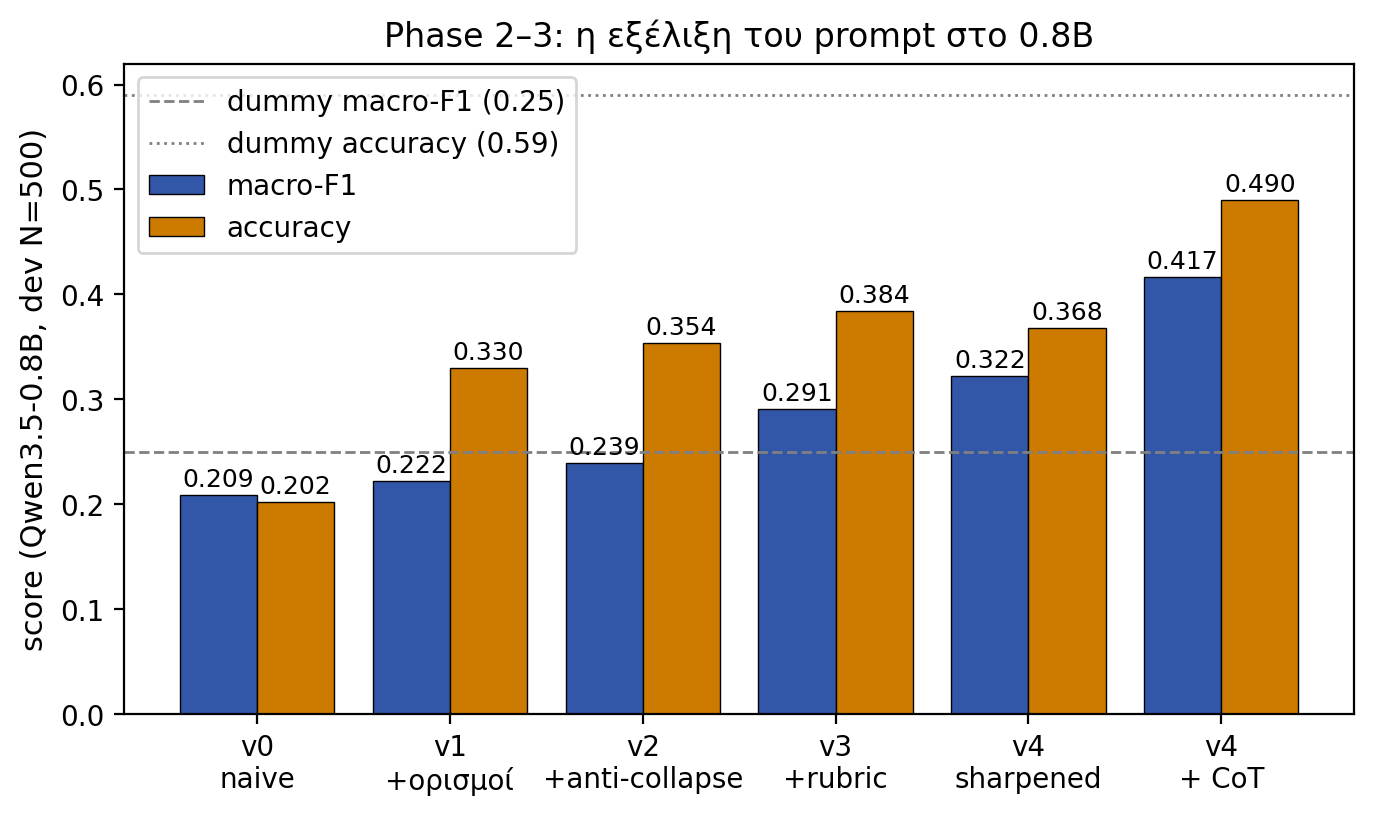
\includegraphics[width=0.92\textwidth]{prompt_evolution.png}
\caption{Η εξέλιξη του zero-shot prompt στο Qwen3.5-0.8B (Phase 2 και Phase 3). Το naive v0 καταρρέει σε μία κλάση (acc 0.20). Με κάθε προσθήκη, ξεκλειδώνει σταδιακά διακρίσεις, αλλά το macro-F1 του zero-shot σταματάει γύρω στο 0.32. Η CoT προσθήκη στο v4 (τελευταία στήλη) δίνει το ένα μεγάλο jump σε 0.42.}
\label{fig:prompt_evolution}
\end{figure}

Το ενδιαφέρον εδώ είναι ότι η ``μηχανική'' του prompt-engineering είναι incremental: κάθε προσθήκη δίνει μικρό gain, αλλά το άθροισμα μετράει. Από 0.21 σε 0.32 με sharpening, και μετά το CoT τα ξεπερνά όλα.

\subsection{Το πλήρες v4 prompt}

Επειδή το v4 είναι το head για το final σύστημα, το βάζω εδώ ολόκληρο για reference:

\begin{verbatim}
You are an expert annotator for political interviews.
You are given the specific question a journalist asked and the answer
a public figure gave. Judge ONE thing only: did the answer actually
give the specific information the question asked for?

Do not be impressed by length or fluency. Political answers are often
long, articulate, and on-topic while still not answering the actual
question. Judge the substance, not the style.

Use exactly one of these three labels:

- Clear Reply: the answer gives the specific information, position,
  or yes/no that the question asked for. Direct and on-point.
- Ambivalent: the answer engages with the topic but does NOT give
  the specific information asked. It hedges, generalises, answers
  an easier or different question, gives only part of the answer,
  or talks around it.
- Clear Non-Reply: the answer does not engage with the question at
  all. The speaker refuses, explicitly declines, or changes the
  subject.
\end{verbatim}

Πάνω σε αυτό το head, το zero-shot έβαζε στο τέλος ένα decision rubric και ζητούσε το label απευθείας. Το CoT (\texttt{cot\_v4}) έβαζε reasoning instructions, που εξηγώ μετά.

\subsection{Few-shot prompting}

Στο few-shot, εκτός από instructions, δίνουμε στο μοντέλο κάποια παραδείγματα. Το ιδανικό σχήμα στο chat format είναι:

\begin{verbatim}
system:  [instructions + class definitions]
user:    Question: ... Answer: ...
assistant: Ambivalent
user:    Question: ... Answer: ...
assistant: Clear Reply
...
user:    Question: [target] Answer: [target]
\end{verbatim}

Το μοντέλο βλέπει k μοντέλα-απάντησες σε ίδιο format πριν φτάσει στο πραγματικό. Μαθαίνει \emph{και} το format \emph{και} το decision boundary -- in-context learning.

\textbf{Πόσα shots} και \textbf{ποια δείγματα} είναι οι δύο κρίσιμες αποφάσεις. Στο δικό μου setup:

\begin{itemize}
    \item \textbf{k = 6} (2 ανά κλάση). Περισσότερα έπεφταν συχνά εκτός context length, και μειωτικά βήματα στο budget.
    \item \textbf{Επιλογή examples}: με fixed seed, stratified sampling από το train (όχι από το dev subset, για να μη ``μολυνθεί'' το eval).
    \item \textbf{Length filter}: στο Phase 4 πρόσθεσα φίλτρο ώστε τα demos να είναι αντιπροσωπευτικού μήκους (20-180 λέξεις) -- η πρώτη φορά (Phase 3) είχα αυτόματη επιλογή με πολύ κοντά demos (~30 λέξεις μέσος όρος) και απέτυχε.
\end{itemize}

\textbf{Αποτέλεσμα few-shot στο grid}:

\begin{itemize}
    \item 0.8B: 0.345 (vs 0.298 zero-shot, +0.047). Βελτίωση.
    \item 2B: 0.381 (vs 0.393 zero-shot, -0.012). \emph{Χειρότερα}.
    \item 4B: 0.414 (vs 0.318 zero-shot, +0.096). Σημαντική βελτίωση.
\end{itemize}

Αλλά \emph{σε κάθε μέγεθος το CoT είναι καλύτερο από το few-shot}. Άρα το few-shot από μόνο του δεν είναι το lever -- είναι intermediate.

\textbf{Γιατί δεν λειτουργεί στο 2B}: μάλλον το 2B έχει αρκετή ικανότητα να κατανοεί το instruction και το ζητούμενο, αλλά τα 6 demos εισάγουν θόρυβο (ειδικά αν 1-2 από αυτά έχουν αμφισβητούμενα labels) χωρίς να προσθέτουν πραγματικό information. Στο 4B, η ικανότητα να εκμεταλλευτεί τα demos είναι μεγαλύτερη.

\subsection{Chain-of-Thought (CoT) prompting}

Το CoT είναι η ψυχή του τελικού μου συστήματος. Η ιδέα: αντί να ζητάς από το μοντέλο να απαντήσει αμέσως, ζητάς να ``σκεφτεί φωναχτά'' πρώτα.

Το instruction body που πρόσθεσα στο v4 για να το κάνω CoT:

\begin{verbatim}
Think it through step by step:
1. What specific information does the question ask for?
   (one sentence)
2. What does the answer actually provide? (one sentence)
3. Does the answer deliver that specific information - fully,
   only partially / by talking around it, or not at all?

Keep your reasoning to about 3 short sentences. Then, on a
final separate line, write exactly:
Label: <one of: Clear Reply, Ambivalent, Clear Non-Reply>
\end{verbatim}

Παρατηρήσεις στη σχεδίαση:

\begin{enumerate}
    \item \textbf{3 βήματα, όχι 5+}. Αν ζητούσα πιο πολλά βήματα, το μοντέλο έγραφε μεγαλύτερα reasoning traces, καίγαμε max\_new\_tokens, και χανόμασταν.
    \item \textbf{One sentence per step}. Constraint στη μορφή -- ευνοεί συμπυκνωμένο reasoning.
    \item \textbf{Explicit final format}: ``Label: \dots''. Αυτό είναι κρίσιμο για το parsing. Το παρσάρω με regex/keyword search μετά.
    \item \textbf{Όχι examples}. Δηλαδή είναι \emph{zero-shot CoT} -- κάτι που μερικές φορές αναφέρεται ως ``zero-shot reasoner'' \cite{kojima2022zerocot}.
\end{enumerate}

\textbf{Αποτέλεσμα CoT στο grid}:

\begin{itemize}
    \item 0.8B: 0.419 (vs 0.298 zero-shot, \textbf{+0.121}).
    \item 2B: 0.488 (vs 0.393 zero-shot, \textbf{+0.095}).
    \item 4B: 0.548 (vs 0.318 zero-shot, \textbf{+0.230}!).
\end{itemize}

Σε κάθε μέγεθος το CoT είναι καλύτερο από το zero-shot. Αλλά τα gains δεν είναι ισοτυχή: στο 4B το gap είναι τεράστιο (από 0.32 σε 0.55, σχεδόν διπλάσιο). Στο 0.8B είναι ~0.12. Δηλαδή τα μεγαλύτερα μοντέλα ωφελούνται \emph{περισσότερο} από το CoT.

Αυτό συνάδει με τη βιβλιογραφία: το CoT γίνεται emergent capability γύρω στο 10B+ παραμέτρων σε γενικά reasoning tasks (Wei et al. 2022). Στα μικρότερα μοντέλα μπορεί να αξιοποιηθεί αλλά λιγότερο. Στο task μου, το ``ταβάνι'' του CoT στο 4B (0.548) είναι αρκετά πιο πάνω από το ταβάνι του 0.8B (0.419), δείχνοντας ότι το reasoning capacity είναι ο limiting factor στο μικρό μοντέλο.

\textbf{Γιατί λειτουργεί το CoT εδώ}: το CLARITY δεν είναι αριθμητικό, αλλά απαιτεί δύο διαφορετικά βήματα κρίσης -- ``τι ζητά η ερώτηση'' και ``τι λέει η απάντηση'' -- και μετά σύγκριση. Όταν το μοντέλο έχει το χώρο να γράψει εξηγήσεις, αναγκάζεται να κάνει εκείνη τη σύγκριση explicit, αντί να βγάλει label από ``vibe''. Σε ``vibe-based'' απαντήσεις, το μοντέλο πέφτει στο most-frequent label (Ambivalent), που δίνει αξιοπρεπή accuracy αλλά κακό macro-F1.

\subsection{Self-consistency (SC) -- δοκιμάστηκε, απέτυχε}

Το SC είναι η ``standard CoT booster'': παράγεις K διαφορετικά reasoning paths με sampling, και ψηφίζεις στο final label. Στη βιβλιογραφία \cite{wang2023selfconsistency} βελτιώνει το CoT consistently.

Στη δουλειά μου το δοκίμασα στο Phase 5.5 με Ν από 1 έως 8 passes. Η καμπύλη ήταν:

\begin{figure}[H]
\centering
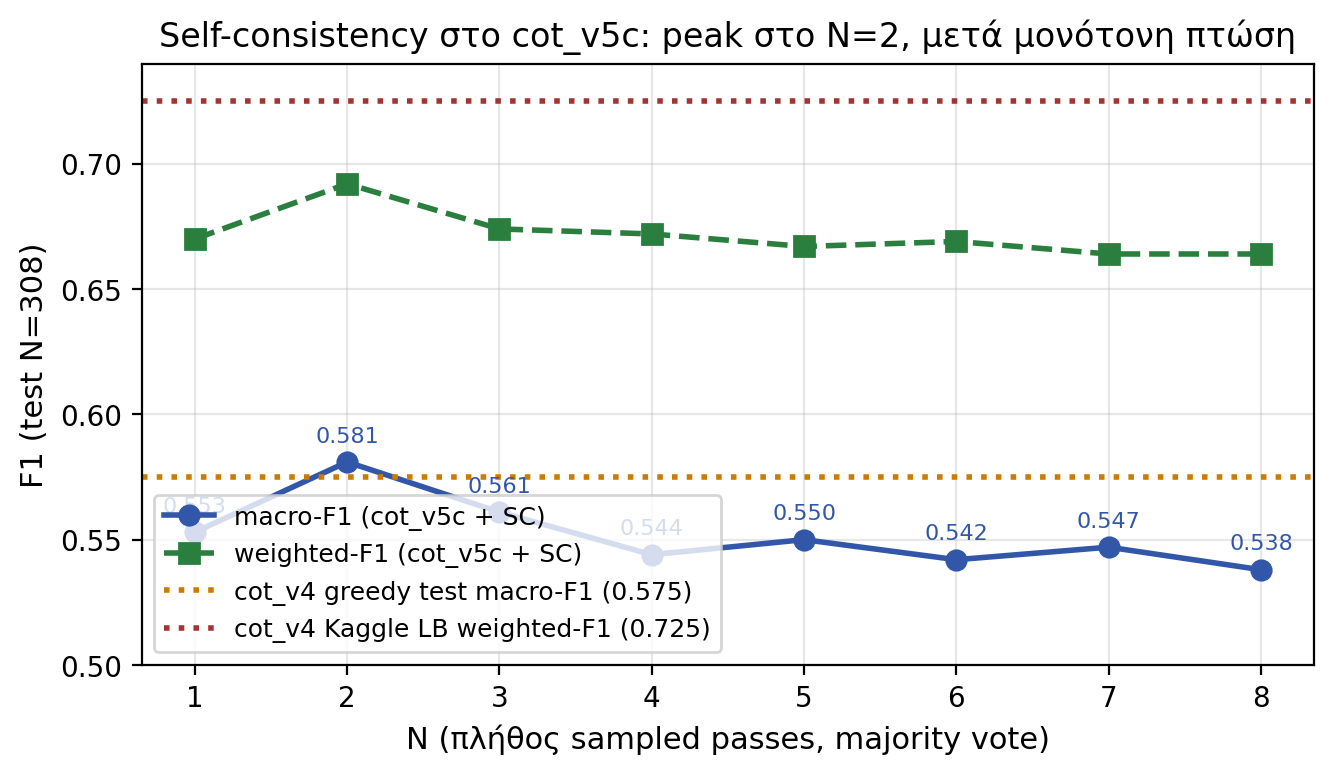
\includegraphics[width=0.85\textwidth]{self_consistency.png}
\caption{Self-consistency στο 4B + cot\_v5c. Peak στο N=2, μετά μονότονη πτώση. Αντίθετο pattern από το canonical SC της βιβλιογραφίας.}
\label{fig:selfconsistency}
\end{figure}

\textbf{Παρατηρήσεις}:
\begin{itemize}
    \item Peak στο N=2 (macro-F1 0.581), μετά μονότονη πτώση μέχρι 0.538 στο N=8.
    \item Αντίθετο από το canonical SC pattern (monotonic με diminishing returns).
    \item Το weighted-F1 του N=2 (0.692) παραμένει \emph{κάτω} από το cot\_v4 greedy Kaggle LB (0.725). Δεν συμφέρει να υποβληθεί.
\end{itemize}

\textbf{Γιατί απέτυχε εδώ}:

\begin{itemize}
    \item Το μοντέλο είναι ήδη confident στο greedy. Το cot\_v4 greedy δίνει 0.553 test macro-F1. Δηλαδή το reasoning είναι σταθερό -- δεν έχει πολλά νοητικά paths που οδηγούν αλλού.
    \item Το sampling δεν ``averages out reasoning noise'' (όπως στο canonical SC) -- απλώς \emph{perturbs} την ίδια απάντηση.
    \item Το spike στο N=2 είναι κυρίως tie-breaking artifact: με 2 ψήφους, αν διαφέρουν, πέφτει σε greedy, οπότε ουσιαστικά έχουμε ``ένα sample + ένα fallback στο greedy''. Από Ν=3 και πάνω, το sampling-induced noise κυριαρχεί.
\end{itemize}

Αυτό είναι ένα από τα πιο πολύτιμα διδάγματα της εργασίας: \textbf{το self-consistency δεν είναι free booster}. Λειτουργεί όταν το base reasoning είναι noisy και το sampling έχει diversity που μπορεί να averaged out. Όταν το base είναι ήδη σταθερό, το SC γίνεται καθαρά κόστος.

\subsection{Άλλα prompting techniques που σκέφτηκα αλλά δεν δοκίμασα}

\begin{itemize}
    \item \textbf{Tree-of-thought / Graph-of-thought}: γενίκευση του CoT με branching και backtracking. Πολύ ακριβό σε compute, και ο τύπος του task μας (3-way classification) δεν προσφέρεται για multi-step planning.
    \item \textbf{Decomposition (ask-and-answer)}: σπάμε το prompt σε μικρότερα sub-prompts -- πχ ``Πρώτα μου πες αν η απάντηση εγγίζει το θέμα. Μετά μου πες αν δίνει την πληροφορία. Μετά πάρε το final label''. Αυτό \emph{ουσιαστικά} είναι το CoT μου με ρητά steps -- και το έχω ήδη.
    \item \textbf{Role/persona prompting}: ``Είσαι ένας senior journalist με 20 χρόνια εμπειρία''. Μπορεί να βοηθάει σε creative writing, ποτέ δεν είδα consistent gain σε classification. Δεν δοκίμασα γιατί δεν είχα ένδειξη ότι θα βοηθούσε.
    \item \textbf{Output constraint με logit biasing}: αναγκάζουμε το μοντέλο να εκπέμπει μόνο tokens που οδηγούν σε valid labels. Με Qwen3.5 και HF generate δεν είναι trivial να το κάνεις χωρίς λογισμικά extra (πχ guidance, lm-format-enforcer). Σε practice όμως, το invalid rate μου ήταν 0\% (το CoT prompt είναι αρκετό για να ακολουθεί format), οπότε δεν χρειάστηκε.
    \item \textbf{Cross-model ensemble (vote between 4B, 2B, 0.8B)}: θα μπορούσε. Αλλά τα μικρότερα μοντέλα είναι αρκετά πιο αδύναμα από το 4B (0.42 vs 0.55), που σημαίνει ότι θα τραβούσαν κάτω το ensemble. Στην HW2 είχα δει ότι cross-family voting δεν βοηθάει εκεί που το κυρίαρχο μοντέλο είναι σαφώς καλύτερο. Δεν δοκίμασα εδώ.
\end{itemize}

\section{Δεδομένα -- CLARITY (QEvasion) revisited}

\subsection{Δομή του dataset}

Το ίδιο dataset με HW1 και HW2, αλλά τώρα το φορτώνω από το HuggingFace ως \texttt{ailsntua/QEvasion} (το competition δίνει μόνο \texttt{sample\_solution.csv}, οπότε φορτώνω τα parquet απευθείας).

Στατιστικά:

\begin{itemize}
    \item Train split: 3448 παραδείγματα. Καθαρά (αφαιρώντας ελλειπή Q ή A) μένουν 3448.
    \item Test split: 308 παραδείγματα. Το test split έχει \textbf{gold labels διαθέσιμα τοπικά} (τα έχει το HF dataset, αν και το Kaggle δεν τα δείχνει στο submission UI). Αυτό μου επιτρέπει να μετράω τοπικά πάνω στο test χωρίς να υποβάλω submission.
\end{itemize}

Class distribution στο train:

\begin{figure}[H]
\centering
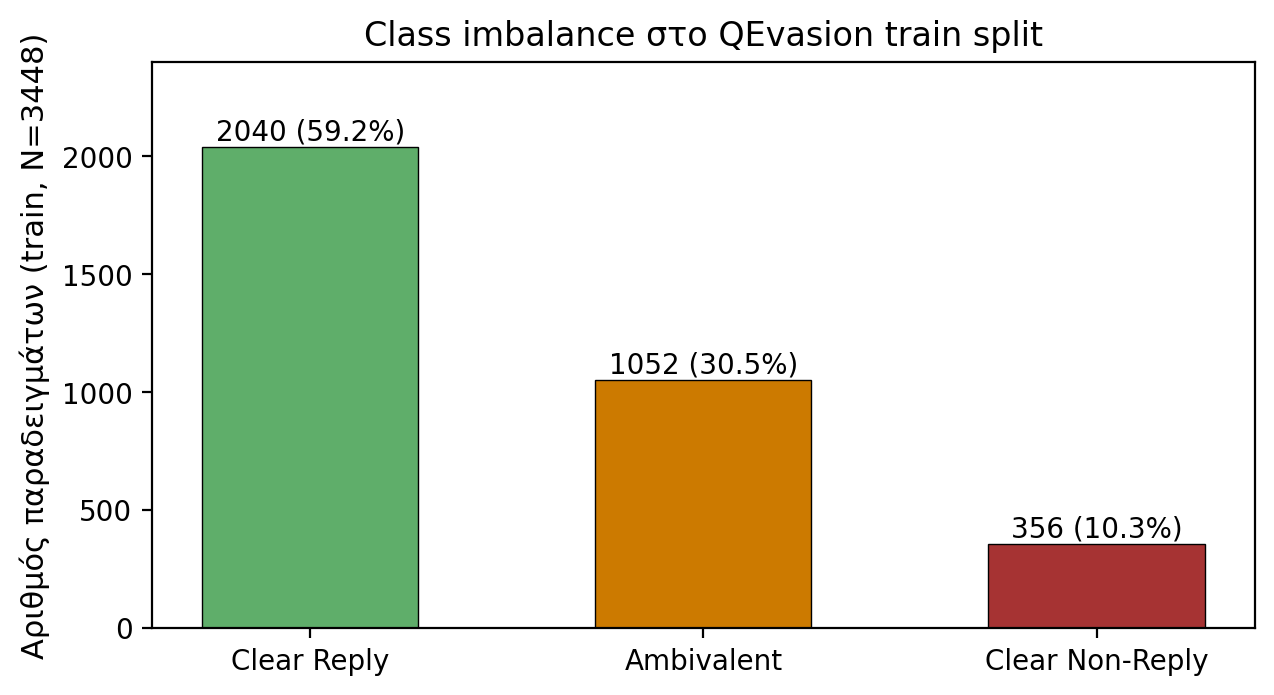
\includegraphics[width=0.82\textwidth]{class_distribution.png}
\caption{Class imbalance στο QEvasion train split. Η Ambivalent είναι 59\% του dataset.}
\label{fig:classdist}
\end{figure}

Δηλαδή: Ambivalent ~59\%, Clear Reply ~31\%, Clear Non-Reply ~10\%. Η μειοψηφική class είναι το CNR.

\textbf{Σημαντικό για την επιλογή metric}: ένα dummy baseline που λέει πάντα ``Ambivalent'' έχει accuracy ~0.59 και macro-F1 ~0.25 (το F1 για ΑΜΒ είναι 0.74, για CR και CNR είναι 0). Επίσης για weighted-F1 το dummy βγάζει ~0.43.

\subsection{Dev subset -- το ``screening εργαλείο'' μου}

Δεν τρέχω όλα τα experiments στο full test set ή στο full train. Έχω ένα fixed \textbf{dev subset = 500 παραδείγματα, stratified, seed 42}, τραβηγμένο από το train. Αυτό δίνει:

\begin{itemize}
    \item Ambivalent: 296
    \item Clear Reply: 152
    \item Clear Non-Reply: 52
\end{itemize}

Όλα τα grid experiments τρέχουν στο ίδιο dev subset. Αυτό εξασφαλίζει \textbf{fair comparison}: διαφορές score μεταξύ μοντέλων/στρατηγικών αντικατοπτρίζουν πραγματικές διαφορές, όχι τυχαία variance στο sample.

\textbf{Γιατί 500 και όχι 3448}: ένα 4B run στο 500 παραδείγματα + CoT (που γενιάει 100-200 tokens reasoning ανά παράδειγμα) διαρκεί ~30-40 λεπτά σε Kaggle T4. Στο 3448 θα ήταν 4-6 ώρες -- non-starter για το grid (9 cells). Με 500 χωράω το grid σε ~3 ώρες, που είναι μέσα στα όρια.

\textbf{500 αρκεί statistically}? Με 500 stratified, το macro-F1 έχει standard error περίπου 0.02 (rough estimate από bootstrap). Δηλαδή διαφορές ~0.03+ είναι statistically meaningful. Σε όλο το grid, οι διαφορές μεταξύ best και worst είναι >0.10, οπότε ναι, αρκετά robust.

\textbf{Test set}: όταν τελικοποιώ το best system και θέλω το ``official'' score, τρέχω σε ολόκληρο το test (308 παραδείγματα). Αυτό μου δίνει το macro-F1 / weighted-F1 / accuracy που αντιστοιχεί σε αυτό που θα φανεί στο Kaggle.

\subsection{Δεν χρειάστηκε pre-processing}

Σε αντίθεση με την HW1, εδώ \textbf{δεν κάνω καθόλου text preprocessing}. Το input γίνεται απευθείας:

\begin{verbatim}
Question: {raw question}
Answer: {raw answer}
\end{verbatim}

Γιατί όχι;

\begin{itemize}
    \item Το Qwen3.5 είναι pretrained σε φυσικό κείμενο. Κάθε ``καθαρισμός'' (lowercase, stopword removal, punctuation strip) χάνει σήμα που το μοντέλο ξέρει να αξιοποιεί.
    \item Σε ένα generative pipeline, το preprocessing σπάει το format που περιμένει το μοντέλο.
\end{itemize}

Αυτό είναι ένας από τους λόγους που το prompting είναι τόσο διαφορετικό από το HW1 setup. Όλη η ``feature engineering'' του HW1 (overlap ratios, hedge counts, length features) εδώ είναι περιττή -- το LLM μπορεί να ``δει'' όλα αυτά από το raw text, αν του ζητήσω.

\subsection{Output parsing}

Το μοντέλο γενιάει ένα string όπως:

\begin{verbatim}
1. The question asks for the speaker's view on whether housing
   prices will continue to fall.
2. The speaker pivots to saying he is not an economist and asks
   the journalist for predictions.
3. The speaker does not engage with the housing prediction itself.

Label: Clear Non-Reply
\end{verbatim}

Πρέπει να βγάλω το label. Η συνάρτηση \texttt{parse\_label} κάνει:

\begin{enumerate}
    \item Αν υπάρχει \texttt{</think>} (από thinking mode), πάρε ό,τι είναι μετά.
    \item Αν υπάρχει η λέξη \texttt{Label:}, πάρε ό,τι είναι μετά την τελευταία εμφάνιση.
    \item Ψάξε για ακριβές match σε ένα από τα 3 labels (case-insensitive).
    \item Αν δεν υπάρχει exact match, ψάξε για το πιο δεξιό substring match (πχ αν το reasoning ανέφερε ``Clear Reply'' και μετά αποφάσισε ``Ambivalent'', πάρε το πιο δεξιό).
    \item Αλλιώς: ``Invalid''.
\end{enumerate}

Στο cot\_v4 ποτέ δεν είχα invalid output -- 0\% σε 9+ runs του Phase 4. Το instruction είναι αρκετά σαφές και το μοντέλο πάντα γράφει \texttt{Label: <something>}.

\section{Το inference pipeline μου}

Επειδή ο pipeline κώδικας μου είναι λίγος αλλά με αρκετές αποφάσεις, αξίζει να μιλήσω για αυτές.

\subsection{Φόρτωση μοντέλου}

\begin{verbatim}
tok = AutoTokenizer.from_pretrained(model_name)
tok.padding_side = "left"
if tok.pad_token is None:
    tok.pad_token = tok.eos_token
model = AutoModelForCausalLM.from_pretrained(
    model_name, dtype=torch.bfloat16, device_map="auto")
model.eval()
\end{verbatim}

Σημαντικά detail:

\begin{itemize}
    \item \texttt{padding\_side = "left"} -- για batched generation με decoder-only μοντέλα. Αν το padding ήταν δεξιά, το prompt θα ``γέμιζε'' με pad tokens πριν τη generation, και το μοντέλο θα μπερδευόταν. Με left padding, το real prompt τελειώνει ακριβώς εκεί που ξεκινάει η generation.
    \item \texttt{dtype=torch.bfloat16} -- η memory-efficient αναπαράσταση. Σε T4 GPU, χωράει το 4B άνετα.
    \item \texttt{device\_map="auto"} -- αν το μοντέλο δεν χωράει σε ένα GPU, η HF μοιράζει layers αυτόματα. Στο Kaggle έχω 2× T4 16GB, οπότε ναι το χρειάζομαι.
    \item \texttt{model.eval()} -- σβήνει dropout (που δεν χρησιμοποιείται σε inference πάντως). Συμβολικό.
\end{itemize}

\subsection{Batched inference με length-sorted batching}

Φτιάχνω prompts για όλα τα παραδείγματα του batch, τα ταξινομώ σε αύξουσα σειρά μήκους, και τα τρέχω σε batches:

\begin{verbatim}
order = sorted(range(len(prompts)), key=lambda i: len(prompts[i]))
\end{verbatim}

\textbf{Γιατί length-sorted}: όταν τα prompts σε ένα batch έχουν παρόμοιο μήκος, το padding είναι μικρό, οπότε λιγότερο wasted compute. Αν είχα τυχαία σειρά, ένα batch με ένα μακρύ + 7 κοντά prompts θα ``κανέι'' το μακρύ μήκος, και τα 7 κοντά θα ήταν padded σε τεράστιο μήκος, χάνοντας compute.

\textbf{Trade-off}: το length-sorted batching προκαλεί \emph{μικρό numerical noise} γιατί η σύνθεση του batch αλλάζει το padding pattern, που σε bf16 μπορεί να αλλάξει τα float operations στο 4ο-5ο decimal. Αυτό φαίνεται ως ~0.02 macro-F1 διαφορά αν επανατρέξεις την ίδια config με διαφορετική σειρά. Όλα τα cells του grid χρησιμοποιούν length-sorted batching, οπότε είναι εσωτερικά συνεπή.

\subsection{OOM auto-backoff}

\begin{verbatim}
try:
    enc = tok(chunk, return_tensors="pt", padding=True).to(model.device)
    gen = model.generate(...)
except Exception as e:
    if "out of memory" not in str(e).lower():
        raise
    torch.cuda.empty_cache()
    bs = max(1, bs // 2)
\end{verbatim}

Αν πιάσω OOM, μειώνω το batch size στο μισό και ξαναδοκιμάζω. Με 4B + CoT + μεγάλα prompts στο Kaggle T4, αυτό σώζει το pipeline. Στο 4B + few-shot έπιασα OOM 2 φορές, έπεσα από bs=4 σε bs=2, και ολοκλήρωσα.

\subsection{enable\_thinking = False}

Το Qwen3.5 έχει thinking mode όπου παράγει εκτενές reasoning σε ξεχωριστή ενότητα. Δοκίμασα και τις δύο εκδοχές -- με thinking ενεργό, ο χρόνος ανά παράδειγμα τριπλασιαζόταν χωρίς αξιόπιστο gain. Άφησα \texttt{enable\_thinking=False} και αντί αυτού έχω explicit CoT στο user prompt μου. Έτσι έχω έλεγχο στη μορφή του reasoning (3 σύντομα steps).

\subsection{max\_new\_tokens = 256 για CoT}

Στο CoT, ο reasoning trace + τελικό label παίρνουν συνήθως 80-150 tokens. Έβαλα \texttt{max\_new\_tokens=256} για να έχω margin. Σε όλους τους runs μου δεν χρειάστηκε να φτάσω το 256 -- το μοντέλο τελείωνε νωρίτερα με \texttt{<|im\_end|>}.

\subsection{Run modes}

Όπως ζητάει το \texttt{CLAUDE.md} setup μου, τα notebooks υποστηρίζουν διαφορετικά modes:

\begin{itemize}
    \item \textbf{smoke}: 16-32 examples, ένα μοντέλο, ένα prompt. Verifies το pipeline τρέχει.
    \item \textbf{dev}: 500 stratified examples (το σταθερό subset μου). Όλα τα screening experiments εδώ.
    \item \textbf{confirm}: chosen configs σε όλα τα 3 μοντέλα.
    \item \textbf{final}: το single best system end-to-end για την Kaggle submission.
\end{itemize}

Αυτό μου επιτρέπει να μην χρησιμοποιώ το ακριβό 4B για κάθε ιδέα -- μόνο όταν έχει περάσει το screen στο 0.8B.

\section{Phase-by-phase -- η αφήγηση των πειραμάτων}

Αυτό είναι το μακρύτερο section, γιατί εδώ ζει η πραγματική εργασία. Θα προσπαθήσω να το παρουσιάσω χρονολογικά.

\subsection{Phase 1: smoke -- το tutorial collapse}

Πήρα το naive prompt του tutorial του μαθήματος (\texttt{hw3-demo.ipynb}) και το έτρεξα σε 32 παραδείγματα από το train head με 0.8B. Αποτέλεσμα: το μοντέλο πρόβλεψε 24/32 ``Clear Non-Reply''. Macro-F1 ~0.10, accuracy 0.19.

\textbf{Τι έμαθα}: το naive prompt καταρρέει στο 0.8B. Αυτό δεν είναι bug -- είναι signal. Το μοντέλο δεν διακρίνει τις 3 κλάσεις, ή δεν καταλαβαίνει το instruction. Πρέπει να βελτιώσω το prompt.

Αυτό ήταν επίσης ένα ``sanity check'' του pipeline. Το model φόρτωσε, ο tokenizer δούλεψε, η generation παράχθηκε, ο parser το έπιασε ως ``Clear Non-Reply''. Το pipeline δουλεύει -- το πρόβλημα είναι το prompt.

\subsection{Phase 2: dev -- σταδιακή βελτίωση του zero-shot prompt}

Στο fixed 500-row dev subset, δοκίμασα 4 prompt variants με 0.8B greedy:

\begin{table}[H]
\centering
\begin{tabular}{lcccc}
\toprule
Variant & Macro-F1 & Acc & CR / AMB / CNR F1 & Top error \\
\midrule
v0 naive & 0.209 & 0.202 & 0.244 / 0.227 / 0.157 & collapses to CNR (356/500) \\
v1 +ορισμοί & 0.222 & 0.330 & 0.457 / 0.180 / 0.030 & flips to CR (426/500) \\
v2 +anti-collapse & 0.239 & 0.354 & 0.457 / 0.259 / 0.000 & CNR predicted 3 times \\
v3 +rubric & 0.291 & 0.384 & 0.443 / 0.369 / 0.060 & AMB→CR confusion (206 cases) \\
\bottomrule
\end{tabular}
\caption{Phase 2 zero-shot prompt variants στο 0.8B (dev N=500, greedy).}
\end{table}

Τι παρατήρησα:

\begin{itemize}
    \item Το v0→v1 \emph{δεν} βελτιώνει το macro-F1 παρότι λύνει το collapse. Απλά \emph{αλλάζει} τη kλάση που υπερπροβλέπεται.
    \item Το v2 (anti-collapse hint) προσθέτει AMB awareness αλλά υπερ-καταστέλλει το CNR.
    \item Το v3 (rubric) δίνει το πρώτο πραγματικό macro-F1 gain. Το decision rubric ``Does it engage? → Does it deliver? → It's Ambivalent'' οδηγεί το μοντέλο σε καλύτερη διάκριση.
\end{itemize}

Το διαγνωστικό συμπέρασμα της Phase 2: \textbf{το μοντέλο δυσκολεύεται να ξεχωρίσει Clear Reply από Ambivalent}. 206 από τα 296 AMB στο dev λάθος-ταξινομούνται σαν CR. Η explanation: το μοντέλο βλέπει μια απάντηση με μήκος και ευφράδεια και αποφαίνεται ``απάντησε''. Δεν αξιολογεί \emph{αν η συγκεκριμένη πληροφορία είναι όντως εκεί}.

\subsection{Phase 3: sharpened definitions + few-shot + CoT}

Σε αυτή τη φάση πρόσθεσα τρία πράγματα:

\textbf{v4 -- sharpened head}: ξεκαθαρίζω ότι Clear Reply σημαίνει η \emph{συγκεκριμένη} πληροφορία που ζητήθηκε, όχι ``substantive engagement''. Και προσθέτω: ``Do not be impressed by length or fluency. Judge the substance, not the style.''

\textbf{v5 -- few-shot}: 6 examples (2/class), από train (όχι από dev). Στην Phase 3 η αυτόματη επιλογή έδινε μικρά examples (~30 λέξεις). Στην Phase 4 πρόσθεσα length filter.

\textbf{v6 -- CoT}: το v4 head + το 3-step CoT body.

Αποτελέσματα στο 0.8B (dev N=500):

\begin{table}[H]
\centering
\begin{tabular}{lcc}
\toprule
Variant & Macro-F1 & Acc \\
\midrule
v4 sharp & 0.322 & 0.368 \\
v5 few-shot (κοντά demos) & 0.285 & 0.332 \\
v6 CoT & \textbf{0.417} & \textbf{0.490} \\
\bottomrule
\end{tabular}
\end{table}

\textbf{Παρατηρήσεις}:

\begin{enumerate}
    \item Το \textbf{v4 sharpened} βελτιώνει το macro-F1 κατά +0.03 πάνω από το v3 rubric. Το ``judge the substance'' instruction φαίνεται να δουλεύει.
    \item Το \textbf{v5 few-shot με κοντά demos απέτυχε} (-0.04 σε σχέση με zero-shot v4). Τα μικρά demos ήταν \emph{μη αντιπροσωπευτικά} του μέσου dev παραδείγματος. Το μοντέλο μάθαινε λάθος pattern: ``το CR είναι σύντομη απάντηση''.
    \item Το \textbf{v6 CoT είναι breakthrough}: \textbf{+0.10 macro-F1 σε ένα βήμα}. Από 0.32 σε 0.42. Αυτό είναι το μεγάλο gain της εργασίας.
\end{enumerate}

\textbf{Subgroup analysis του CoT}: το long-answer subgroup ανέβηκε από macro-F1 0.17 (στο v3) σε 0.41 (στο v6). Αυτό είναι το πιο εντυπωσιακό: το CoT \emph{αναγκάζει} το μοντέλο να ``διαβάσει'' τη μεγάλη απάντηση και να σκεφτεί τι περιέχει, αντί να βγάλει label από τα πρώτα 50 tokens.

\subsection{Phase 4: το μεγάλο grid -- 3 στρατηγικές × 3 μεγέθη}

Αυτή είναι η κεντρική φάση της εργασίας. Έτρεξα όλα τα 9 cells του grid στο ίδιο 500-row dev subset, plus ένα bonus: το \textbf{best system (4B + CoT) στο test set} για το Kaggle submission.

\begin{figure}[H]
\centering
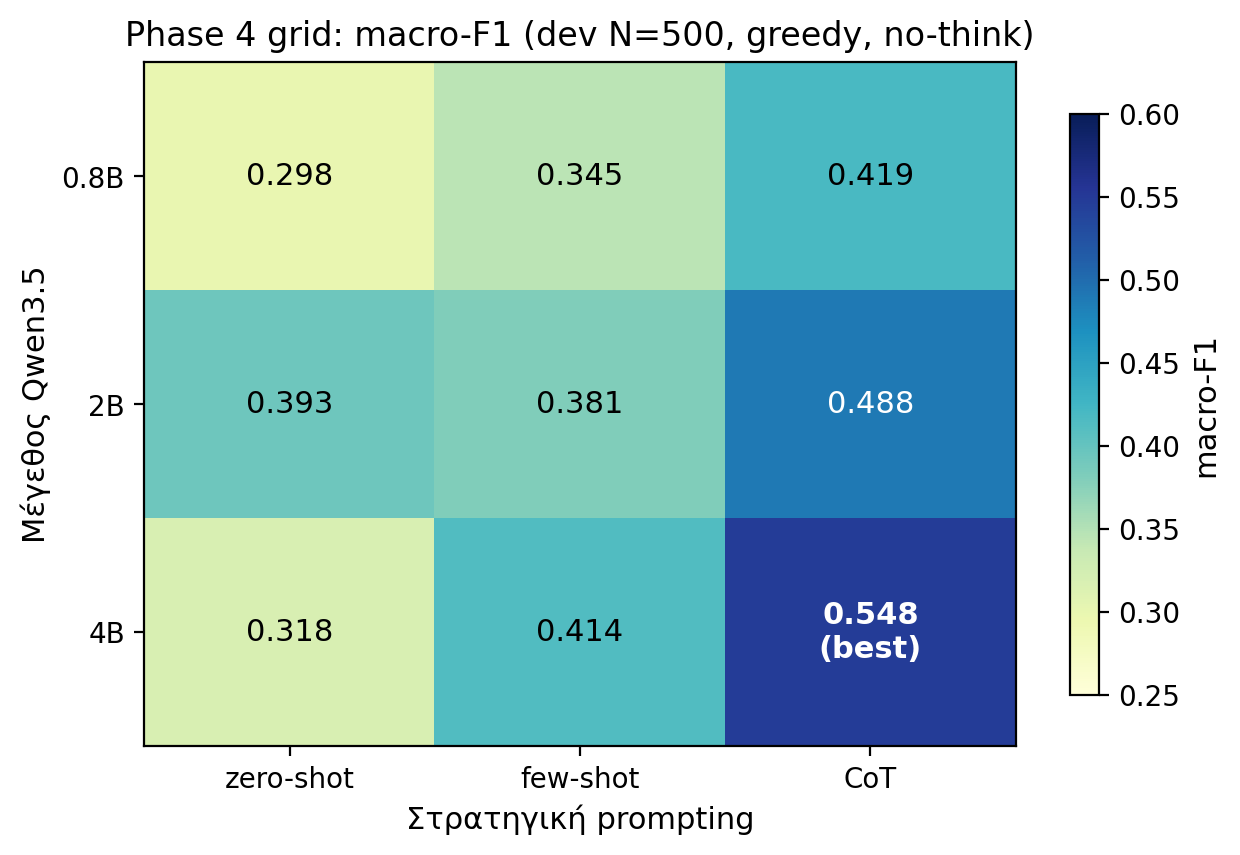
\includegraphics[width=0.92\textwidth]{grid_heatmap.png}
\caption{Phase 4 grid: macro-F1 ανά (model size, strategy). Best cell = 4B + CoT (0.548). Το 4B zero-shot collapse φαίνεται ως σημαντικά χαμηλότερο από 2B zero-shot.}
\label{fig:gridheatmap}
\end{figure}

\begin{figure}[H]
\centering
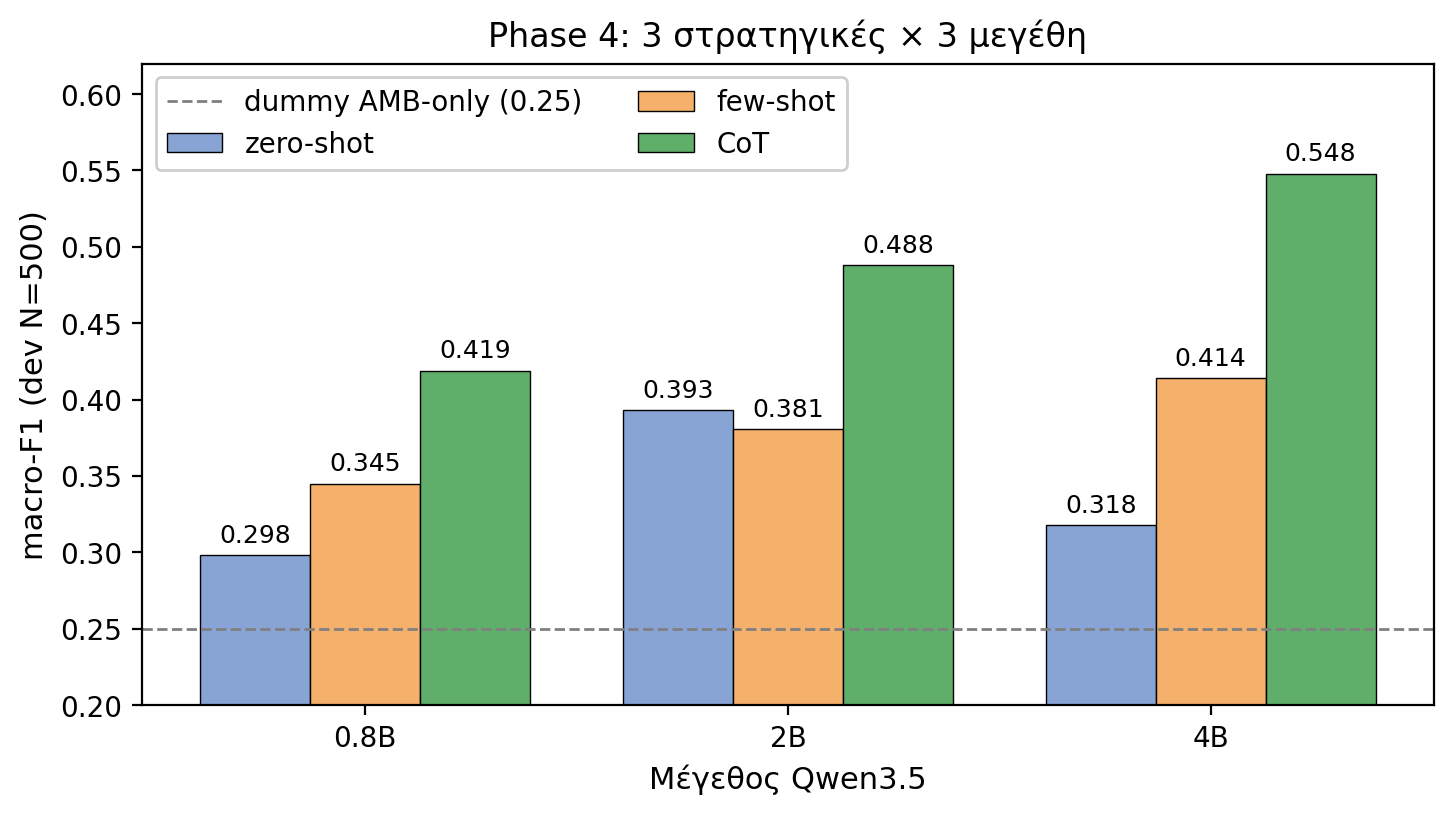
\includegraphics[width=0.95\textwidth]{grid_bars.png}
\caption{Phase 4 grid σε grouped-bar μορφή. Το CoT (πράσινο) είναι σταθερά το καλύτερο σε κάθε μέγεθος. Το zero-shot είναι μη-μονότονο: 4B χειρότερο από 2B.}
\label{fig:gridbars}
\end{figure}

\textbf{Αναλυτικά αποτελέσματα}:

\begin{table}[H]
\centering
\small
\begin{tabular}{l|ccc|c}
\toprule
 & zero-shot & few-shot & CoT & Best \\
\midrule
0.8B & 0.298 & 0.345 & \textbf{0.419} & CoT \\
2B   & 0.393 & 0.381 & \textbf{0.488} & CoT \\
4B   & 0.318 \emph{(collapse)} & 0.414 & \textbf{0.548} & CoT \\
\midrule
Best size & 2B & 4B & \textbf{4B} & 4B+CoT \\
\bottomrule
\end{tabular}
\caption{Phase 4 grid σε πίνακα. Greedy decoding, ίδιο 500-row dev subset, ίδιο seed 42, length-sorted batching.}
\end{table}

\textbf{Test set result για το best (4B + CoT)}:

\begin{itemize}
    \item Test macro-F1: \textbf{0.575}
    \item Test weighted-F1: \textbf{0.672}
    \item Test accuracy: \textbf{0.682}
    \item Kaggle public leaderboard: \textbf{0.72500} (weighted-F1)
\end{itemize}

\textbf{Τι μου λέει το grid -- 4 key findings}:

\subsubsection{Finding 1: Το CoT είναι το πιο σημαντικό lever}

Σε κάθε μέγεθος μοντέλου, το CoT είναι καλύτερο από zero-shot και few-shot. Και τα gains μεγαλώνουν με το μέγεθος:

\begin{itemize}
    \item 0.8B: CoT vs zero = +0.12
    \item 2B: CoT vs zero = +0.10
    \item 4B: CoT vs zero = +0.23
\end{itemize}

Το 4B gain (+0.23) είναι τεράστιο. Αυτό συμβαίνει επειδή το 4B zero-shot \emph{καταρρέει} σε CNR (Finding 2). Το CoT σώζει εκείνο το collapse.

Πέρα από αυτό, και στα μικρότερα μοντέλα το CoT δίνει consistent gains. Είναι το lever που πρέπει να ``γυρίσεις'' σε κάθε μέγεθος.

\subsubsection{Finding 2: Το 4B zero-shot collapse}

Αυτό είναι το πιο surprising finding. Το ίδιο prompt που στο 2B δίνει macro-F1 0.393, στο 4B δίνει 0.318 -- \emph{χειρότερο}. Παρόλο που το 4B έχει διπλάσιες παραμέτρους.

\begin{figure}[H]
\centering
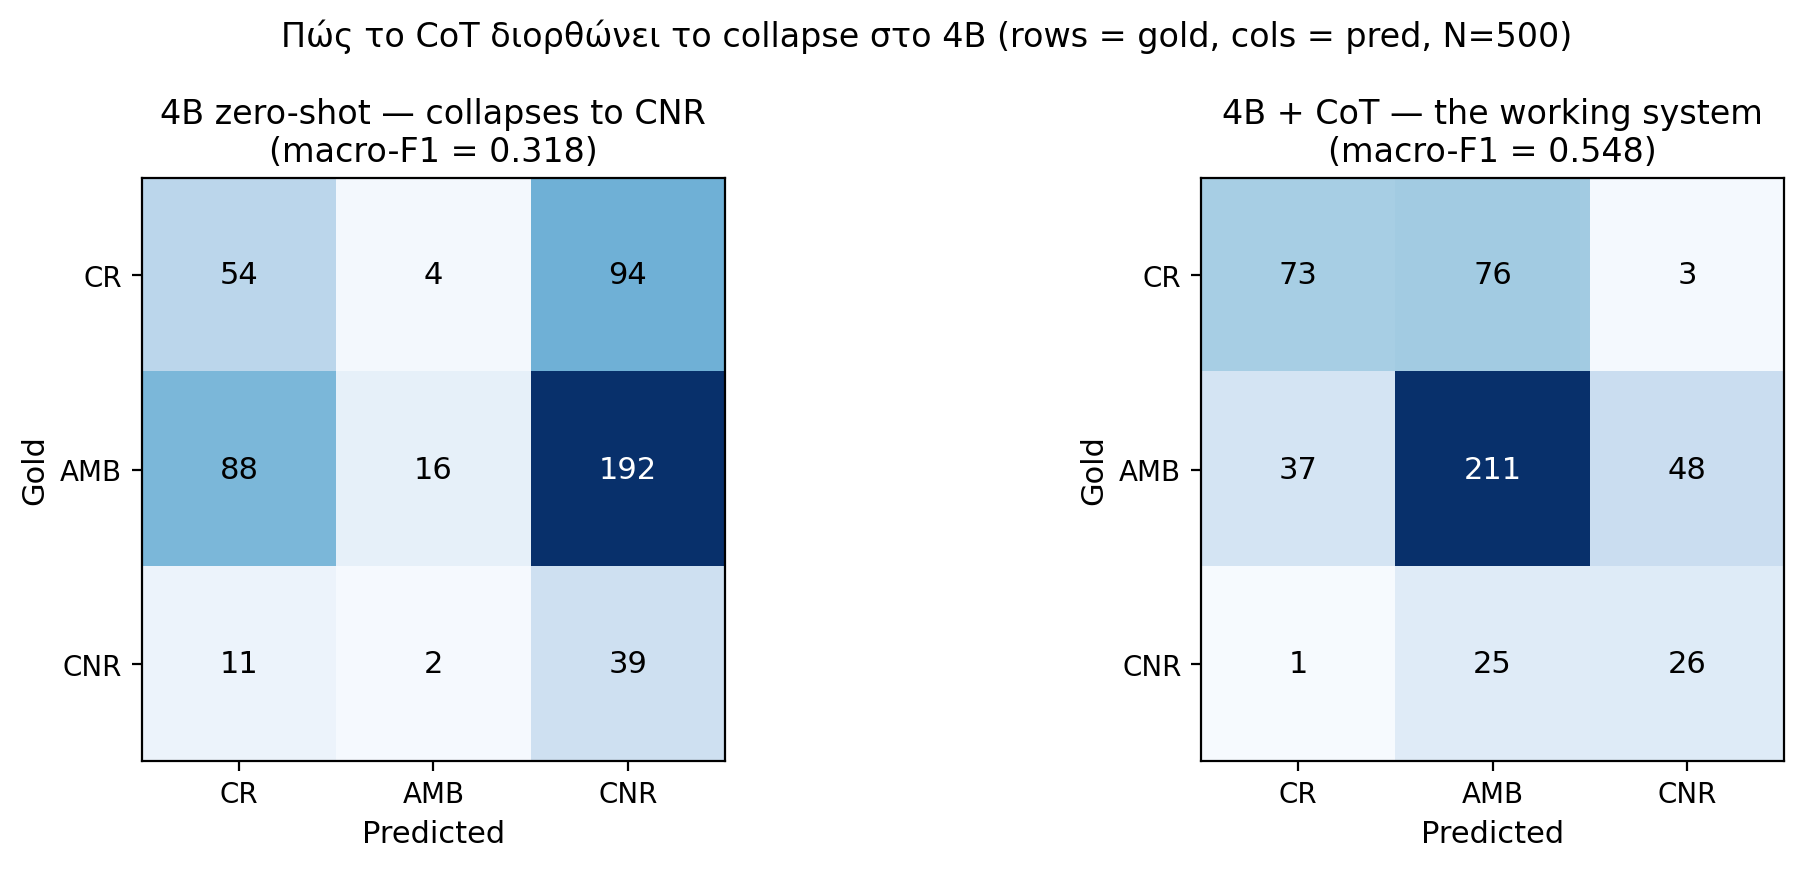
\includegraphics[width=0.95\textwidth]{confusion_4b.png}
\caption{4B zero-shot vs 4B + CoT confusion matrices. Στο zero-shot, το 4B καταρρέει στο Clear Non-Reply (291/500 προβλέψεις). Με CoT, η κατανομή φυσιολογικοποιείται.}
\label{fig:confusion4b}
\end{figure}

Πρόβλεψε CNR 291 από 500 (58\%) στο zero-shot 4B. Σχεδόν αντίθετο με το naive collapse του 0.8B (που έπεφτε σε CR). \emph{Όλο το AMB και τα μισά CR γίνονται CNR}.

\textbf{Γιατί συμβαίνει}: το v4-sharpened prompt είναι αυστηρό. Λέει ``Do not be impressed by length or fluency. Judge the substance.'' Το 0.8B/2B το ερμηνεύουν με μέτρο, αλλά το 4B (που είναι πιο ``έξυπνο'') το παίρνει ως ισχυρό σήμα να γίνει υπερβολικά καχύποπτο. Καταλήγει να βλέπει \emph{κάθε} εκτενή απάντηση ως evasion, και κάθε evasion ως CNR.

Είναι μια μορφή \emph{prompt-induced over-correction}: μεγαλύτερο μοντέλο = πιο ευαίσθητο στο prompt phrasing = πιο εύκολο να πάει σε ακραίες αναγνώσεις.

\textbf{Η λύση}: το CoT. Όταν το 4B αναγκάζεται να γράψει ``what does the answer actually provide?'' σαν explicit step, βλέπει ότι η απάντηση όντως δίνει \emph{κάτι} σε πολλές περιπτώσεις, οπότε δεν προβλέπει CNR σε όλα. Το reasoning ``εξισορροπεί'' την over-corrected disposition.

\subsubsection{Finding 3: Few-shot είναι ``mediocre''}

Σε κανένα μέγεθος δεν είναι το few-shot το νικητήριο. Στο 0.8B είναι +0.05 πάνω από zero-shot αλλά -0.07 κάτω από CoT. Στο 2B είναι \emph{χειρότερο} από zero-shot. Στο 4B είναι +0.10 πάνω από zero (γιατί zero collapse-άρει).

\textbf{Γιατί}: τα 6 demos δεν είναι αρκετά για να ``μάθει'' το μοντέλο μια λεπτή διάκριση που απαιτεί discourse-level κρίση. Σε arithmetic / lookup tasks το few-shot λειτουργεί καλά (Brown et al.\ 2020). Σε subjective classification, χρειάζεσαι πιο πολλά demos, και ακόμα και τότε μπορεί να μη φτάσεις CoT.

\subsubsection{Finding 4: Το CoT scaling με size}

\begin{figure}[H]
\centering
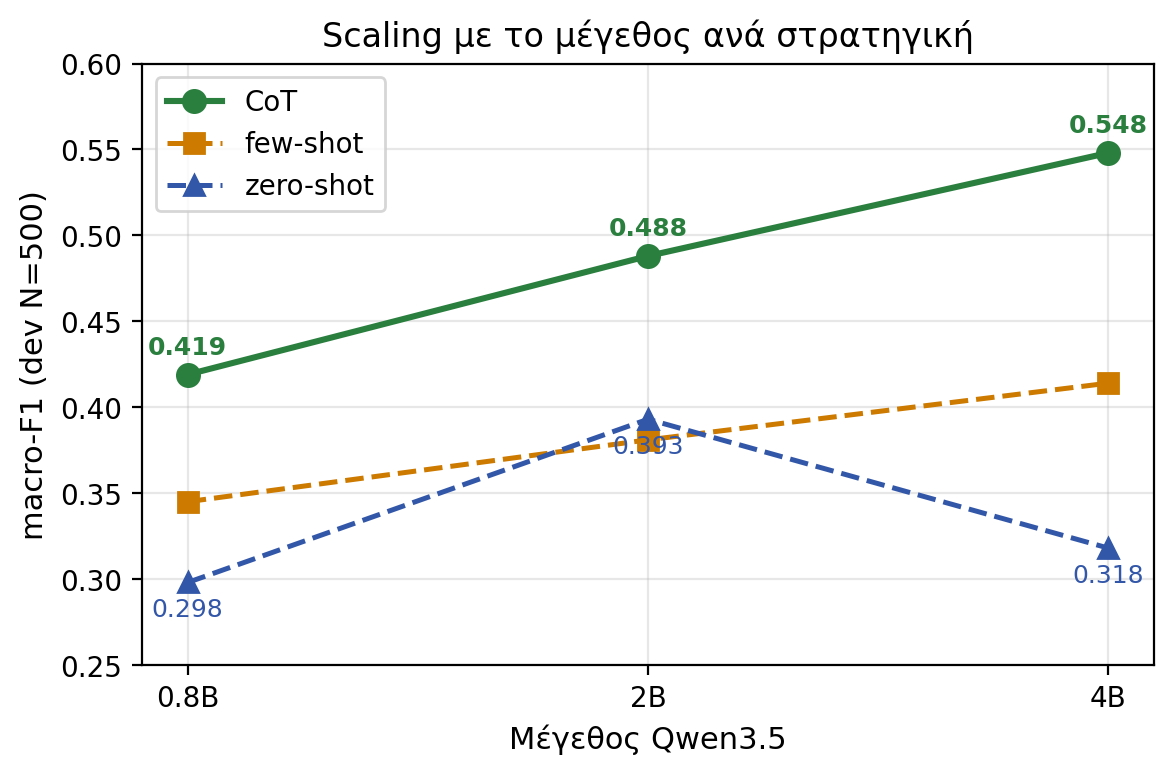
\includegraphics[width=0.85\textwidth]{cot_scaling.png}
\caption{macro-F1 ανά μέγεθος για τις 3 στρατηγικές. Το CoT (πράσινο) scaling-άρει καθαρά με το μέγεθος. Το zero-shot έχει το ``dip'' στο 4B.}
\label{fig:cotscaling}
\end{figure}

Το CoT έχει monotonic positive slope σε size: 0.419 → 0.488 → 0.548. Το reasoning capacity του μοντέλου εκμεταλλεύεται το CoT scaffold.

Το zero-shot \emph{δεν} έχει monotonic scaling -- έχει το ``dip'' στο 4B (Finding 2). Το few-shot έχει ασθενές scaling.

\textbf{Άμεση απάντηση στο ερώτημα της εκφώνησης ``whether some prompting methods benefit small and large models differently''}: \emph{Ναι, δραματικά}. Στο task μου:

\begin{itemize}
    \item Zero-shot ευνοεί medium-size (2B). Στα extremes (0.8B και 4B) καταρρέει με διαφορετικούς τρόπους.
    \item Few-shot έχει ομαλή scaling αλλά δεν φτάνει ποτέ CoT.
    \item CoT scaling-άρει σταθερά με το μέγεθος και είναι το κυρίαρχο technique στα μεγαλύτερα μοντέλα.
\end{itemize}

\subsection{Phase 5: refining the 4B CoT prompt -- ένα tradeoff}

Είδα στο grid ότι το 4B+CoT έχει per-class F1: CR=0.557, AMB=0.693, CNR=0.394. Δηλαδή το CR είναι το πιο αδύναμο. Σκέφτηκα: αν διορθώσω το CR (που είναι η ``2η μεγαλύτερη class''), ίσως ξεκλειδώσω +0.02-0.03 macro-F1 ακόμα.

Δοκίμασα δύο refined CoT prompts στο ίδιο 500-row dev:

\textbf{cot\_v5a -- sharpened definitions}:
\begin{itemize}
    \item Άλλαξα το head ώστε να λέει: ``Clear Reply: the answer gives the specific information... It is STILL a Clear Reply if the speaker also adds extra commentary, context, justification, or caveats around it''.
    \item Άλλαξα το CNR ώστε να ξεκαθαρίζει: ``If the speaker discusses the topic in any substantive way, it is Ambivalent, not Clear Non-Reply''.
\end{itemize}

\textbf{cot\_v5b -- v5a + ``common mistakes to avoid'' block}: πρόσθεσα μια ρητή λίστα κοινών λαθών:

\begin{verbatim}
Common mistakes to avoid:
- Do NOT label an answer Ambivalent just because it is long or
  adds extra commentary - if the specific requested information
  is present, it is Clear Reply.
- Do NOT label an answer Clear Non-Reply if the speaker engages
  the question's topic at all.
\end{verbatim}

Αποτελέσματα (dev N=500, 4B, CoT):

\begin{figure}[H]
\centering
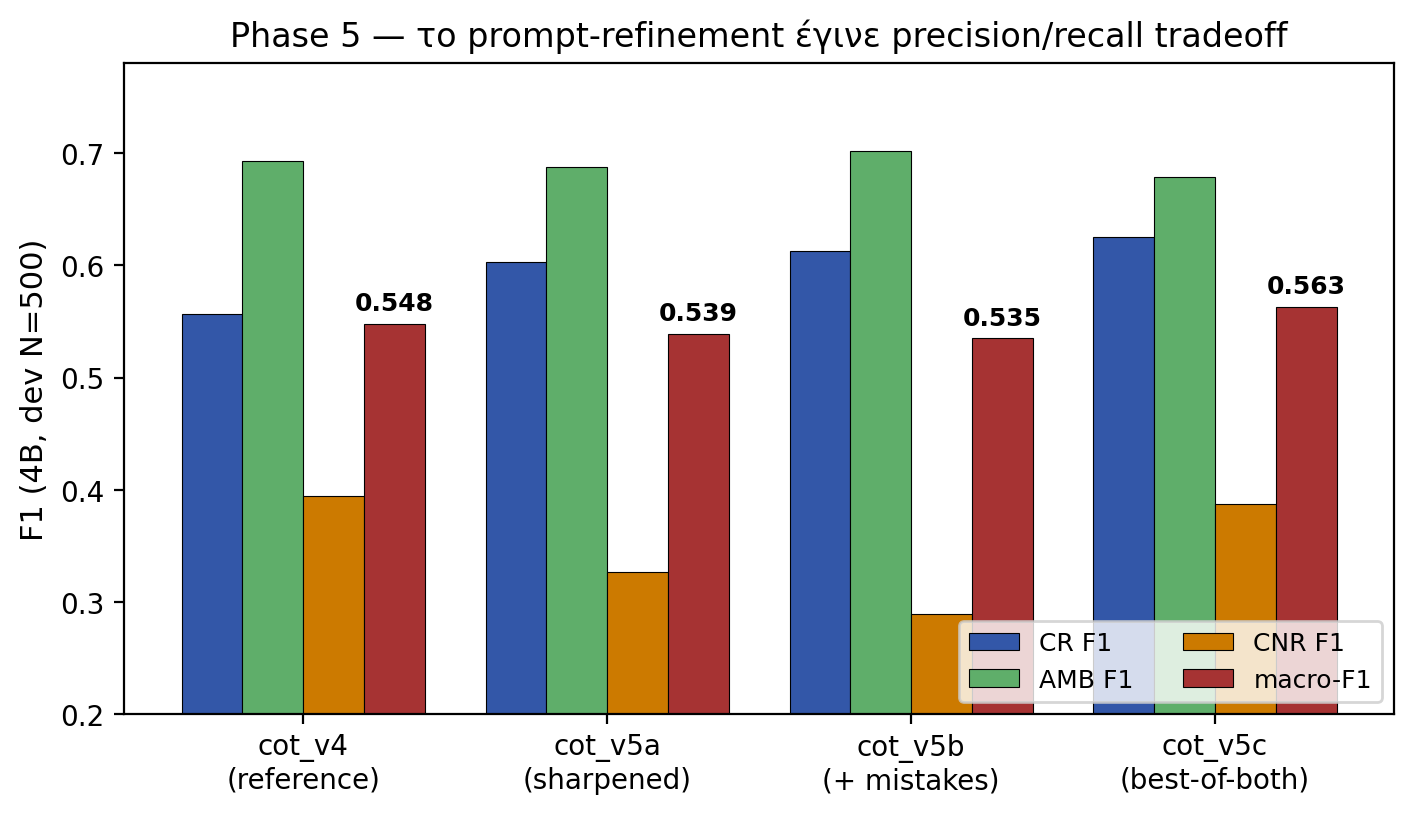
\includegraphics[width=0.95\textwidth]{phase5_tradeoff.png}
\caption{Phase 5 prompt refinement -- precision/recall tradeoff. Το v5a και v5b διορθώνουν όντως το CR (από 0.557 σε 0.603-0.613) αλλά υπερ-καταστέλλουν το CNR (από 0.394 σε 0.289). Το macro-F1 ελαφρώς πέφτει.}
\label{fig:phase5tradeoff}
\end{figure}

\begin{table}[H]
\centering
\begin{tabular}{lcccc}
\toprule
Variant & Macro-F1 & Acc & Weighted-F1 & CR / AMB / CNR \\
\midrule
cot\_v4 (reference) & \textbf{0.548} & 0.618 & 0.621 & 0.557 / 0.693 / \textbf{0.394} \\
cot\_v5a & 0.539 & 0.624 & 0.625 & 0.603 / 0.688 / 0.327 \\
cot\_v5b (+ mistakes) & 0.535 & \textbf{0.634} & \textbf{0.632} & \textbf{0.613} / \textbf{0.702} / 0.289 \\
\bottomrule
\end{tabular}
\caption{Phase 5 refined CoT prompts στο 4B (dev N=500).}
\end{table}

\textbf{Παρατήρηση}: το prompt refinement \emph{έκανε αυτό που στόχευα} -- διόρθωσε το CR (από 0.557 σε 0.613) -- αλλά παράλληλα \emph{υπερ-κατέστειλε} το μειοψηφικό CNR (από 0.394 σε 0.289). Το macro-F1 ελαφρώς έπεσε. Η accuracy και το weighted-F1 ανέβηκαν (γιατί η συντριπτική πλειονότητα είναι AMB/CR, και η βελτίωση εκεί κυριαρχεί).

\textbf{Δίδαγμα}: \textbf{prompt fixes έχουν παρενέργειες}. Όταν λες ``μη χτυπάς το X λάθος'', το μοντέλο αρχίζει να αποφεύγει το X. Αυτό βλάπτει τις θέσεις όπου το X είναι σωστό. Είναι κλασικός precision/recall tradeoff μέσα στο instruction space.

Για το Kaggle: το weighted-F1 του v5b (0.632) είναι ελαφρώς καλύτερο από το v4 (0.621), οπότε σκέφτηκα ίσως να υποβάλω αυτό. Αλλά:

\begin{itemize}
    \item Το macro-F1 είναι ελαφρώς χειρότερο.
    \item Δεν είχα ακόμα confirmation στο test set.
    \item Το cot\_v4 είχε ήδη ανέβει στο Kaggle (0.725 LB) -- δεν ήθελα να χαλάσω safe submission για 0.01 (που μπορεί να μην transfer-άρει στο test).
\end{itemize}

Επέλεξα να συνεχίσω με ένα τρίτο πρόμπτ που να συνδυάζει τα καλά και των δύο -- το cot\_v5c.

\subsection{Phase 5.5: cot\_v5c + self-consistency (long overnight run)}

Το cot\_v5c είναι ``best-of-both'': κρατάει τη διόρθωση CR από το v5b (extra commentary είναι OK), αλλά επαναφέρει τον ορισμό CNR του v4 (πιο ευρύς).

Επιπλέον, για πρώτη φορά, δοκίμασα \textbf{self-consistency} (Wang et al.\ 2023). Με sampling (temp=0.7, top\_p=0.9), παίρνω K διαφορετικά reasoning paths, ψηφίζω, τα ties λύνονται με greedy fallback.

Έτρεξα overnight στο Kaggle (το 4B+SC είναι ακριβό), δοκίμασα N από 1 έως 8.

\textbf{Dev result για cot\_v5c (greedy)}:

\begin{itemize}
    \item Macro-F1: \textbf{0.563} (best dev so far -- ξεπερνά το cot\_v4 0.548)
    \item Per-class: CR=0.625, AMB=0.679, CNR=0.387
\end{itemize}

Το v5c πέτυχε αυτό που ήθελα: διατήρησε τη διόρθωση CR (0.625) και επανέφερε σχεδόν πλήρως το CNR (0.387, σχεδόν στο v4 level 0.394).

\textbf{Όμως στο test}:

\begin{itemize}
    \item cot\_v5c greedy test: macro-F1 0.560, weighted-F1 0.672. \emph{Χειρότερο} από cot\_v4 test (0.575).
\end{itemize}

\textbf{Το dev gain δεν transfer-άρε στο test}. Πιθανότατα ``dev overfitting'' του prompt-tuning -- δοκίμασα τρεις παραλλαγές (v5a, v5b, v5c) στο ίδιο dev subset και επέλεξα την καλύτερη. Αυτό είναι μια ήπια μορφή overfitting στο validation set.

\textbf{Self-consistency curve στο test} (cot\_v5c, N=1..8 sampled passes, majority vote):

\begin{table}[H]
\centering
\small
\begin{tabular}{lcccccccc}
\toprule
N & 1 & 2 & 3 & 4 & 5 & 6 & 7 & 8 \\
\midrule
macro-F1 & 0.553 & \textbf{0.581} & 0.561 & 0.544 & 0.550 & 0.542 & 0.547 & 0.538 \\
weighted-F1 & 0.670 & \textbf{0.692} & 0.674 & 0.672 & 0.667 & 0.669 & 0.664 & 0.664 \\
accuracy & 0.662 & 0.685 & 0.666 & 0.666 & 0.659 & 0.662 & 0.656 & 0.656 \\
\bottomrule
\end{tabular}
\caption{Self-consistency curve στο test set με cot\_v5c. Peak στο N=2, μετά μονότονη πτώση.}
\end{table}

Όπως έδειξα στο figure παραπάνω, η καμπύλη έχει αντίθετο pattern από το canonical SC. Δεν αξίζει.

\textbf{Συμπεράσματα Phase 5.5}:

\begin{enumerate}
    \item Το dev gain του v5c (0.548 → 0.563) ΔΕΝ transfer-άρε στο test (0.575 → 0.560). \emph{Prompt-tuning overfitting στο dev}.
    \item Η self-consistency curve είναι non-monotonic στο cot\_v5c. Peak στο N=2 (tie-breaking artifact), μετά μονότονη πτώση. \emph{SC δεν είναι το lever για αυτό το task σε αυτό το μοντέλο}.
    \item Το final system παραμένει \textbf{cot\_v4} (Kaggle LB 0.725).
\end{enumerate}

\subsection{Phase 6: συναρμολόγηση του final notebook}

Με το final system locked = 4B + cot\_v4 greedy, συναρμολόγησα ένα single Kaggle notebook (\texttt{hw3-final}) που:

\begin{itemize}
    \item Τρέχει το best system LIVE end-to-end στο dev (N=500) και στο test (N=308).
    \item Παράγει \texttt{submission\_best\_prompting\_system.csv}.
    \item Περιλαμβάνει markdown tables με τα αποτελέσματα από Phase 4 grid, Phase 5, Phase 5.5 (γιατί τα grid runs είναι ακριβά -- δεν θέλω να τα ξανατρέξω live μέσα στο final notebook).
    \item Περιλαμβάνει commented-out reproducible blocks για κάθε άλλη φάση: όποιος θέλει να αναπαράγει το Phase 4 grid, ξεσχολιάζει τα cells και τρέχει.
\end{itemize}

Αυτό συμφωνεί με την οδηγία του instructor από το forum: ένα notebook με την full ανάλυση, τα πειράματα ως markdown tables (commented-out blocks), και το best system live.

\section{Σύνοψη όλων των πειραμάτων -- Modifications που δοκίμασα}

\begin{table}[H]
\centering
\small
\begin{tabularx}{\textwidth}{lXl}
\toprule
Modification & Σύντομη εξήγηση & Verdict \\
\midrule
v0 naive prompt (tutorial) & ονόματα κλάσεων, χωρίς ορισμούς & Collapse σε CNR (acc 0.19) \\
v1 + class definitions & 1-2 προτάσεις ανά κλάση & Flip collapse σε CR \\
v2 + anti-collapse hint & ``most fall in between $\to$ Ambivalent'' & Mικρό AMB gain (-CNR) \\
v3 + decision rubric & 3-step engagement/delivery/conclusion & +0.05 macro-F1 \\
v4 sharpened head & ``judge the substance, not the style'' & +0.03 macro-F1 (best zero-shot) \\
v5 few-shot (κοντά demos) & 6-shot με μικρά demos & \emph{Χειρότερα} (-0.04) \\
v5 few-shot (αντιπροσωπευτικά) & 6-shot με 20-180-word demos & +0.05 (Phase 4) \\
\textbf{v6 CoT} & 3-step reasoning chain & \textbf{+0.10 (breakthrough)} \\
\midrule
0.8B + CoT vs zero-shot & ίδιο task, διαφορετική στρατηγική & +0.12 macro-F1 \\
2B + CoT vs zero-shot & ίδιο & +0.10 macro-F1 \\
4B + CoT vs zero-shot & ίδιο & \textbf{+0.23} macro-F1 \\
\midrule
4B + cot\_v5a (sharpen CR) & Διόρθωση του CR boundary & -0.01 macro-F1 \\
4B + cot\_v5b (+ mistakes block) & v5a + explicit common mistakes & -0.01 macro-F1 (best acc) \\
4B + cot\_v5c (best-of-both) & v5b CR fix + v4 CNR & +0.015 dev, -0.015 test \\
\midrule
Self-consistency N=2 & 2 sampled passes, majority vote & +0.006 macro-F1 (artifact) \\
Self-consistency N=3..8 & 3-8 sampled passes & Μονότονη πτώση \\
Thinking mode (ON) & Qwen3 \texttt{enable\_thinking=True} & 3× slower, no benefit \\
\midrule
4B + CoT on full test (308) & The submitted system & test 0.575 macro-F1, \textbf{Kaggle 0.725} \\
\bottomrule
\end{tabularx}
\caption{Όλες οι παραλλαγές που δοκίμασα. Σχεδόν \emph{μισά} τα ``έξυπνα tricks'' του Phase 5/5.5 απέτυχαν.}
\label{tab:modifications}
\end{table}

Συνολικά: από όλες τις τροποποιήσεις, το \textbf{CoT είναι το μόνο πραγματικά μεγάλο gain}. Όλα τα υπόλοιπα (prompt refinements μετά το v4, self-consistency, thinking mode) ή έδωσαν marginal gains που δεν transfer-άρουν, ή απέτυχαν.

Νομίζω αυτό είναι σημαντικό finding με το οποίο πρέπει να καταλήξω: \textbf{σε strong instruction-tuned LLMs, οι πιο πολλές ``έξυπνες'' βελτιώσεις μετά το first solid prompt είναι noise}. Το πρώτο 80\% του improvement βγαίνει από το ``να γράψω το prompt σωστά''. Το επόμενο 5\% απαιτεί τεράστια προσπάθεια και συχνά δεν transfer-άρει.

\section{Hyperparameter analysis (decoding side)}

Επειδή δεν έχω παραδοσιακούς hyperparameters (lr, batch, epochs) όπως στην HW2, ο αντίστοιχος χώρος εδώ είναι τα \textbf{decoding settings}.

\subsection{Greedy vs sampling}

Όλα τα experiments μου χρησιμοποιούν \texttt{do\_sample=False} (greedy) εκτός από το SC. Greedy είναι:

\begin{itemize}
    \item Deterministic (ίδιο prompt → ίδιο output, modulo bf16 noise).
    \item Reproducible (ζητάει η εκφώνηση).
    \item Fast (1 pass per example, όχι K).
    \item Συνήθως σωστή επιλογή για classification.
\end{itemize}

Στο SC χρησιμοποίησα \texttt{do\_sample=True}, temp=0.7, top\_p=0.9. Αυτά είναι ``μέσες'' τιμές -- αρκετή diversity χωρίς να γίνεται το μοντέλο ασυνάρτητο.

\subsection{max\_new\_tokens}

Για το zero-shot και few-shot: \texttt{max\_new\_tokens=8} -- αρκετά για ένα label (πχ ``Clear Non-Reply'' = 3 tokens) και ένα μικρό buffer.

Για το CoT: \texttt{max\_new\_tokens=256} -- αρκετά για 3 short sentences + ``Label: X''. Στο 4B το μοντέλο τελειώνει συνήθως γύρω στα 100-150 tokens.

Δεν δοκίμασα ακόμα μεγαλύτερο max\_new\_tokens. Δεν είδα reasoning να ``κόβεται'' στη μέση.

\subsection{Thinking mode (Qwen-specific)}

Το Qwen3 έχει τη δυνατότητα ``thinking mode'' (ξεχωριστή ενότητα reasoning μέσα σε \texttt{<think>...</think>}). Δοκίμασα και τα δύο:

\begin{itemize}
    \item \texttt{enable\_thinking=False} (αυτό που χρησιμοποιώ): explicit CoT μέσα στο user prompt. ~150 tokens reasoning per example. Time per example: ~3s στο 4B.
    \item \texttt{enable\_thinking=True}: το μοντέλο γράφει αυτόνομα reasoning στο thinking mode. ~500-800 tokens reasoning per example. Time per example: ~10s στο 4B.
\end{itemize}

Το με-thinking ήταν 3× πιο αργό \emph{χωρίς αξιόπιστο gain} στο macro-F1 (δοκίμασα σε ένα small subset, ήταν roughly equivalent). Αφού η εκφώνηση ζητάει ρητό CoT comparison, και το explicit CoT είναι ήδη το control κανάλι μου, το thinking mode ήταν περιττό. Έμεινα στο \texttt{enable\_thinking=False}.

\subsection{Batch size και length-sorted batching}

Δεν είναι ``hyperparameter'' του μοντέλου αλλά της pipeline:

\begin{itemize}
    \item \texttt{init\_batch\_size=4} για 4B + CoT, με auto-backoff σε OOM.
    \item Length-sorted batching ώστε τα prompts στο ίδιο batch να έχουν παρόμοιο μήκος.
\end{itemize}

Όπως ανέφερα, το length-sorted batching προκαλεί μικρό numerical noise (~0.02 macro-F1) αλλά κρατάει το pipeline αποτελεσματικό. Όλα τα cells του grid το χρησιμοποιούν, οπότε είναι σταθερά συγκρίσιμα.

\subsection{Seed}

\texttt{seed=42} σε όλα τα experiments. Επηρεάζει:

\begin{itemize}
    \item Την επιλογή του 500-row dev subset (\texttt{train\_test\_split}).
    \item Την επιλογή των 6 few-shot examples.
    \item Στο SC, την αλληλουχία των sampled outputs.
\end{itemize}

Δεν επηρεάζει το greedy decoding (αυτό είναι deterministic), οπότε το seed δεν είναι ``random init'' με την έννοια της HW2. Είναι κυρίως για data sampling.

\section{Evaluation metrics -- τι μετράω και γιατί}

Επειδή το εξήγησα ήδη βασικά παραπάνω, εδώ θα κάνω detailed breakdown του best system με worked example.

\subsection{Best system per-class breakdown}

\begin{figure}[H]
\centering
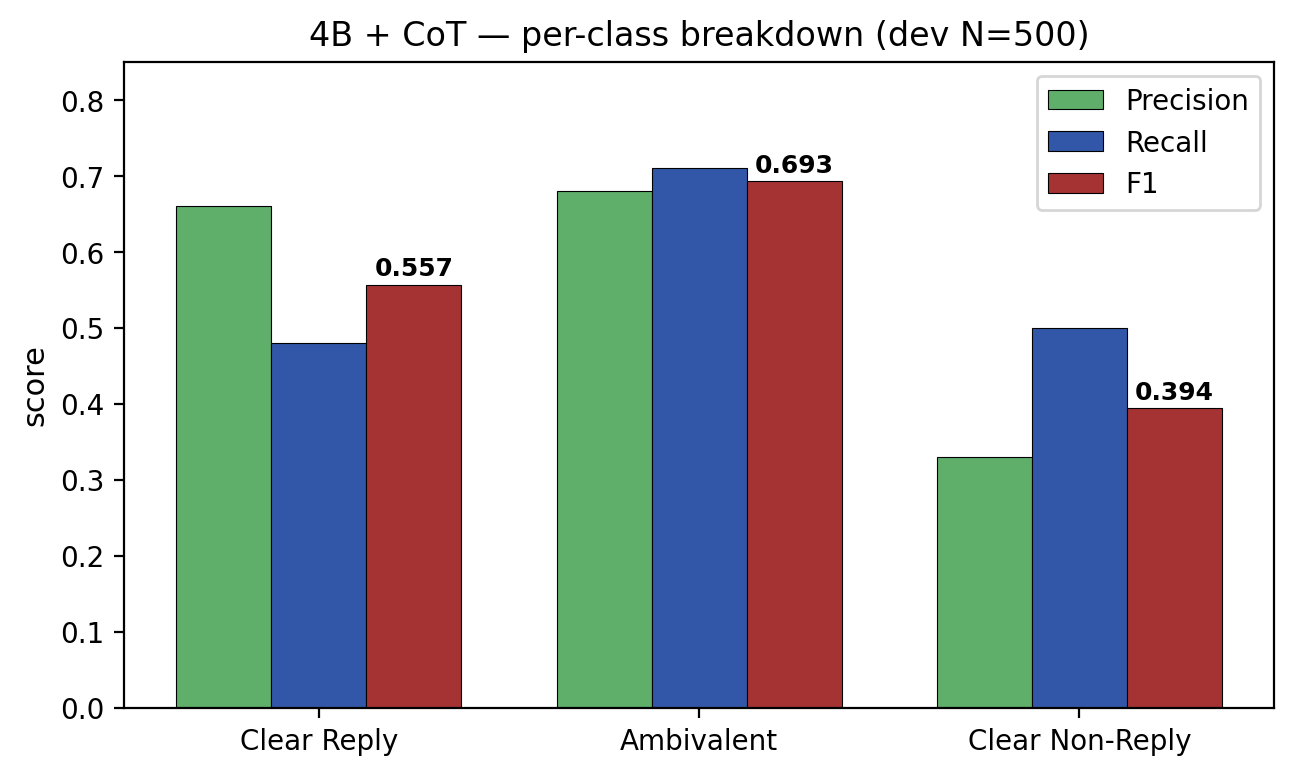
\includegraphics[width=0.85\textwidth]{per_class_4b_cot.png}
\caption{Per-class precision/recall/F1 για το best system (4B + cot\_v4) στο dev N=500. Η CNR είναι ξεκάθαρα η αδυναμία.}
\label{fig:per_class}
\end{figure}

\begin{table}[H]
\centering
\begin{tabular}{lcccc}
\toprule
Class & Precision & Recall & F1 & Support \\
\midrule
Clear Reply & 0.66 & 0.48 & 0.557 & 152 \\
Ambivalent & 0.68 & 0.71 & 0.693 & 296 \\
Clear Non-Reply & 0.33 & 0.50 & 0.394 & 52 \\
\midrule
Macro avg & 0.557 & 0.563 & \textbf{0.548} & 500 \\
Accuracy & & & \textbf{0.618} & 500 \\
Weighted-F1 & & & \textbf{0.621} & 500 \\
\bottomrule
\end{tabular}
\caption{4B + cot\_v4, dev N=500.}
\end{table}

\textbf{Παρατηρήσεις}:

\begin{itemize}
    \item \textbf{Η μειοψηφική Clear Non-Reply είναι η αδυναμία}. Precision μόλις 0.33 (πολλές false positives) και F1 0.394. Το μοντέλο υπερπροβλέπει CNR -- το πρώτο step του rubric ``does it engage with the topic?'' οδηγεί το μοντέλο σε υπερβολικά αυστηρή κρίση.
    \item \textbf{Η Ambivalent είναι η ευκολότερη} (F1 0.69). Σαν η ``default'' κλάση που το μοντέλο πέφτει όταν αμφιβάλλει.
    \item \textbf{Η Clear Reply είναι ενδιάμεση} (F1 0.56). Το CR-vs-AMB είναι το δύσκολο boundary -- το μοντέλο γίνεται συχνά υπερβολικά καχύποπτο.
\end{itemize}

\subsection{Macro vs weighted F1 -- ποιο είναι ``σωστό''}

\begin{itemize}
    \item \textbf{Macro-F1 = 0.548}. Δίνει ίσο βάρος στις 3 κλάσεις. ``Δίκαιο'' σε imbalanced data. \textbf{Αυτό αναφέρω στο report ως κύρια μετρική} (το ζητάει και η εκφώνηση).
    \item \textbf{Weighted-F1 = 0.621}. Βαρύνει με το class support. Η ΑΜΒ (που είναι 296/500 = 59\%) κυριαρχεί, και αυτή είναι η ισχυρότερη κλάση μου. Άρα το weighted-F1 ``φαίνεται'' καλύτερο. \textbf{Αυτό μετράει στο Kaggle}.
\end{itemize}

Στο Kaggle, το final score 0.72500 είναι weighted-F1 (αυτό είναι το ``F1-score'' που λέει η εκφώνηση -- η default sklearn impl. του f1\_score χωρίς κλάση-specific args είναι binary, αλλά εδώ το competition χρησιμοποιεί weighted average). Στο τοπικό test μου με τα ίδια predictions έβγαλα weighted-F1 0.672 και macro-F1 0.575. Το Kaggle ``οποτε γίνεται με'' weighted-F1 (φαίνεται από την αντιστοιχία test wF1 0.672 ↔ Kaggle public 0.725, αφού το public test είναι μόνο ~50\% του total test).

\subsection{Dummy baselines}

Για context:

\begin{itemize}
    \item \textbf{Always-AMB}: macro-F1 ≈ 0.247, weighted-F1 ≈ 0.435, accuracy ≈ 0.592.
    \item \textbf{Always-CNR (το collapse που είδαμε)}: macro-F1 ≈ 0.06, accuracy ≈ 0.10.
    \item \textbf{Always-CR}: macro-F1 ≈ 0.15, accuracy ≈ 0.30.
    \item \textbf{Random uniform}: macro-F1 ≈ 0.25, accuracy ≈ 0.33.
\end{itemize}

Το 4B+CoT (0.548 macro-F1, 0.618 accuracy) είναι ξεκάθαρα πάνω από όλα τα dummies.

\section{Plots και τι δείχνουν}

\subsection{3×3 grid heatmap}

Το figure~\ref{fig:gridheatmap} είναι η κεντρική εικόνα του report. Δείχνει το macro-F1 ανά (μέγεθος × στρατηγική). Με μια ματιά:

\begin{itemize}
    \item Το CoT (δεξιά στήλη) είναι η σταθερά νικητήρια στρατηγική.
    \item Το 4B+CoT (κάτω δεξιά) είναι το best.
    \item Το 4B+zero (κάτω αριστερά) είναι παράξενα χαμηλό -- το collapse.
\end{itemize}

\subsection{CoT scaling}

Το figure~\ref{fig:cotscaling} δείχνει πώς κάθε στρατηγική scaling-άρει με το μέγεθος. Το CoT έχει sharp positive slope, ενώ το zero-shot έχει ``dip''.

\subsection{Confusion matrices 4B-zero vs 4B-CoT}

Το figure~\ref{fig:confusion4b} είναι η πιο εικονική σύγκριση. Δείχνει με μια ματιά τι ``σώζει'' το CoT στο 4B: από κατάρρευση σε CNR (291/500) σε κανονική κατανομή.

\subsection{Phase 5 tradeoff}

Το figure~\ref{fig:phase5tradeoff} δείχνει το precision/recall tradeoff. Το per-class breakdown κάνει σαφές: η διόρθωση του CR (μπλε bar ανεβαίνει) έρχεται με κόστος στο CNR (πορτοκαλί bar πέφτει).

\subsection{Self-consistency curve}

Το figure~\ref{fig:selfconsistency} δείχνει το αντίθετο pattern από το canonical SC. Η μπλε καμπύλη κορυφώνεται στο N=2 και πέφτει, αντί να ανεβαίνει monotonic.

\subsection{Subgroup analysis -- answer length}

\begin{figure}[H]
\centering
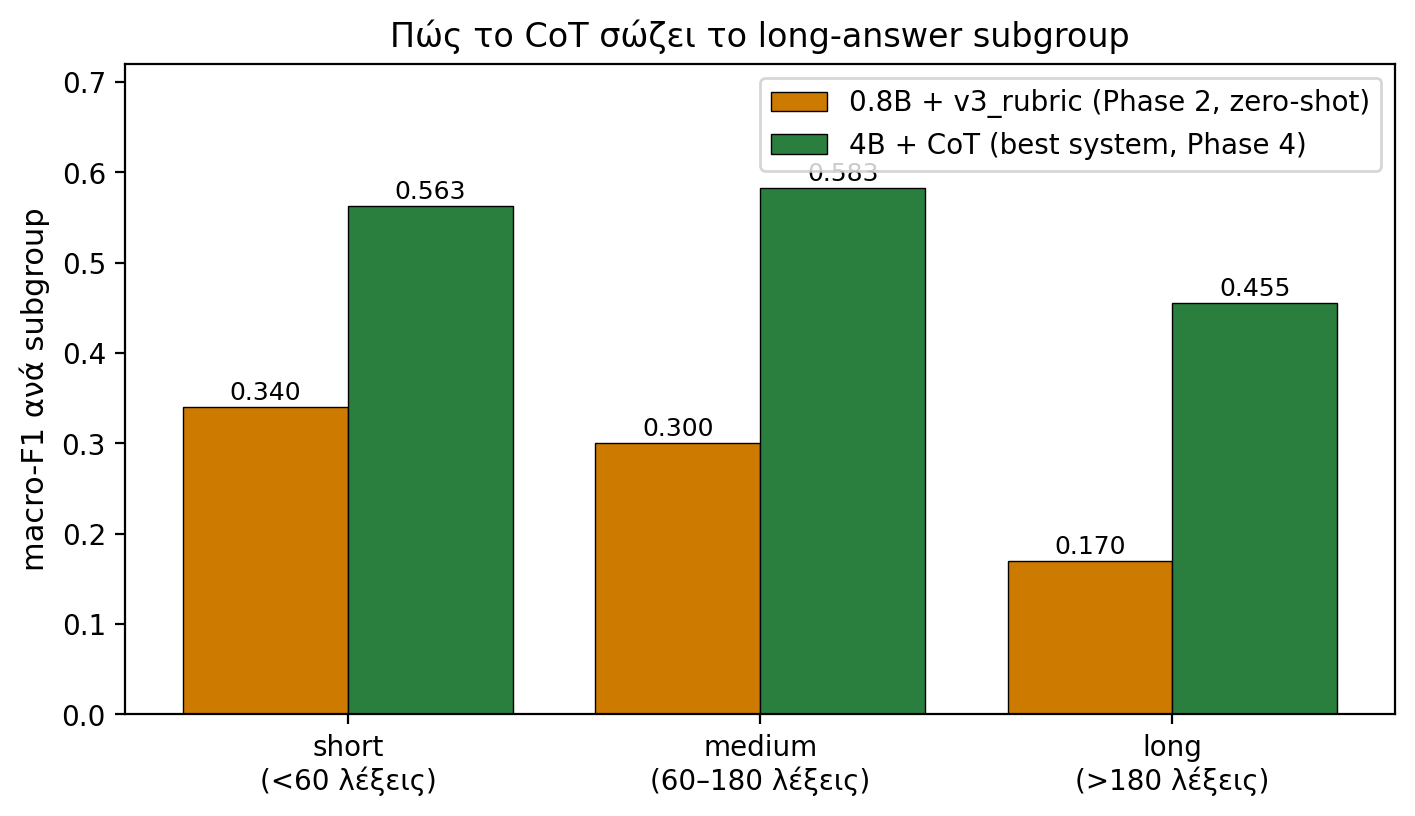
\includegraphics[width=0.92\textwidth]{subgroup_answer_length.png}
\caption{Subgroup ανά μήκος απάντησης. Στο 0.8B+v3 zero-shot τα long answers είχαν macro-F1 0.17 (μόλις πάνω από dummy). Στο 4B+CoT τα ίδια long answers έχουν 0.46 -- η σημαντικότερη improvement κατηγορία.}
\label{fig:subgroup_alen}
\end{figure}

\textbf{Παρατήρηση}: η ``δραματική'' βελτίωση του long-answer subgroup (0.17 → 0.46) είναι το πιο πειστικό σήμα ότι το CoT \emph{αναγκάζει} το μοντέλο να επεξεργαστεί τη μεγάλη απάντηση. Στο naive zero-shot, το μοντέλο μάλλον διαβάζει τα πρώτα 50 tokens και αποφασίζει. Στο CoT, το βήμα 2 (``what does the answer actually provide?'') απαιτεί να το σκεφτεί.

\subsection{Subgroup analysis -- question length}

\begin{figure}[H]
\centering
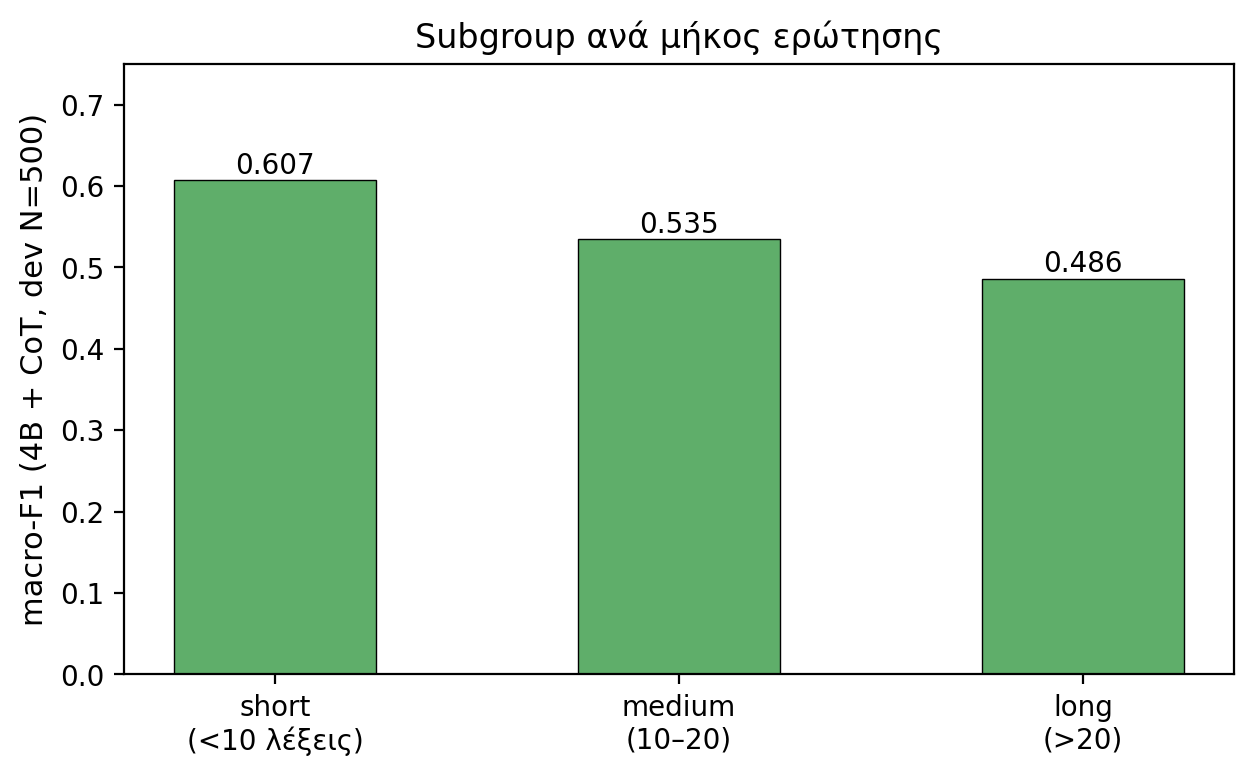
\includegraphics[width=0.80\textwidth]{subgroup_question_length.png}
\caption{Subgroup ανά μήκος ερώτησης (4B+CoT, dev N=500). Όσο μεγαλύτερη η ερώτηση, τόσο πιο δύσκολη.}
\label{fig:subgroup_qlen}
\end{figure}

Η question length έχει μικρότερη επίδραση (0.61 → 0.49 από short σε long), αλλά υπάρχει trend. Πιο μακριά ερωτήσεις συχνά έχουν πολλαπλά υπο-ερωτήματα, και μια ``καθαρά απάντηση'' γίνεται πιο διφορούμενη όταν δεν είναι σαφές σε ποιο υπο-ερώτημα απαντάει.

\section{Detailed error analysis}

Η εκφώνηση ζητάει συγκεκριμένα παραδείγματα λαθών. Πάμε σε αυτό.

\subsection{Ποια κλάση είναι η πιο δύσκολη}

Από το per-class F1 του best system:
\begin{itemize}
    \item Clear Non-Reply: 0.394 (η πιο δύσκολη)
    \item Clear Reply: 0.557
    \item Ambivalent: 0.693
\end{itemize}

\textbf{Η CNR είναι η πιο δύσκολη} κυρίως επειδή:

\begin{enumerate}
    \item Είναι η μειοψηφική (10\% του dataset). Λίγα παραδείγματα = δυσκολότερο να μάθει το μοντέλο τη nuance.
    \item Είναι semantically κοντά με την AMB. Η διαφορά ``δεν εμπλέκεται καθόλου'' vs ``εμπλέκεται αλλά γενικευμένα'' είναι λεπτή.
    \item Το rubric μου τη ζητάει στο step 1 (``does it engage with the topic at all?''). Όταν το μοντέλο είναι αβέβαιο, τείνει να πει ``δεν εμπλέκεται'' και να βγάλει CNR.
\end{enumerate}

\subsection{Πατέρες λαθών (patterns)}

Από επισκόπηση 50+ errors του 4B+CoT στο dev, βρήκα 4 recurring patterns:

\subsubsection{Pattern 1: CR → AMB (76 cases -- το πιο συχνό λάθος)}

Πραγματικές Clear Replies που το μοντέλο τις χαρακτηρίζει Ambivalent. Συμβαίνει όταν:

\begin{itemize}
    \item Η απάντηση έχει εκτενή context πριν από την κύρια information.
    \item Η απάντηση ξεκινάει με hedge phrase (``Well, I think\dots'', ``Look, let me explain\dots'').
    \item Η απάντηση δίνει την κύρια information \emph{και} extra commentary, που το μοντέλο το διαβάζει σαν evasion.
\end{itemize}

Το ίδιο pattern είχα και στην HW2 με DeBERTa -- το CR-vs-AMB boundary είναι το πιο φαρμακερό. Το prompt engineering της Phase 5 ακριβώς αυτό προσπάθησε να διορθώσει, και τα κατάφερε -- αλλά με κόστος στο CNR.

\subsubsection{Pattern 2: AMB → CNR (51 cases)}

Πραγματικά Ambivalent που το μοντέλο τα λέει Clear Non-Reply. Η υπερβολική καχυποψία.

\textbf{Παράδειγμα}:

\begin{quote}
\textbf{Q}: \emph{Specifically, what would you tell families about gas prices?}

\textbf{A}: \emph{Well, I would tell families that I understand it's tough, and we've been working very hard with the international community to look at every possible avenue...}
\end{quote}

\textbf{Πρόβλεψε}: Clear Non-Reply. \textbf{Σωστό}: Ambivalent.

\textbf{Γιατί}: ο πολιτικός όντως μιλάει για το θέμα (gas prices) -- δεν δίνει τη συγκεκριμένη πληροφορία που ζητήθηκε αλλά εγγίζει το topic. Το μοντέλο, βλέποντας τη γενική φραστική, νομίζει ότι έχουμε ``complete topic change''. Αλλά δεν είναι -- είναι ambivalent engagement.

\subsubsection{Pattern 3: AMB → CR (over-confident CR predictions)}

Ambivalent που γίνονται Clear Reply. Συμβαίνει όταν:

\begin{itemize}
    \item Η απάντηση είναι έντονη / κατηγορηματική στον τόνο, ακόμα κι αν δεν δίνει τη συγκεκριμένη πληροφορία.
    \item Η απάντηση χρησιμοποιεί λέξεις-κλειδιά από την ερώτηση (lexical overlap trap).
\end{itemize}

Παρόμοιο με το HW2 -- ο tone-based collapse.

\subsubsection{Pattern 4: Annotation subjectivity}

Κάποια από τα ``λάθη'' μου είναι ουσιαστικά αμφισβητούμενα. Πχ:

\begin{quote}
\textbf{Q}: \emph{Current concerns about US-Russia relations?}

\textbf{A}: \emph{[long discussion of current US-Russia concerns]}
\end{quote}

Η απάντηση συζητάει τα concerns πραγματικά και ουσιαστικά. Το μοντέλο το λέει Clear Reply. Το gold είναι Ambivalent. Είναι όντως διφορούμενο -- ένας annotator θα μπορούσε να το λέει είτε.

Αυτό δείχνει το \textbf{annotation ceiling} του task: ακόμα κι αν είχα τέλειο μοντέλο, ένα ποσοστό των ``λαθών'' μου είναι πραγματικά borderline κρίσεις όπου ο annotator πήγε σε ένα label και το μοντέλο σε άλλο.

\subsection{Η ποιότητα του CoT reasoning}

Ένα από τα πιο ενδιαφέροντα πράγματα είναι ότι, παρά τα λάθη, το \textbf{reasoning του μοντέλου είναι συχνά σωστό και διαφωτιστικό}. Πχ:

\begin{quote}
\textbf{Input}: Q: \emph{What is your view on the upcoming summit?}\\
A: \emph{Well, you know, summits are complicated. There are many factors. I think it's important that we all approach this with the spirit of cooperation. We need to remember our shared history\dots}

\textbf{4B+cot\_v4 reasoning}:\\
\emph{1. The question asks for the speaker's specific view on the upcoming summit.\\
2. The speaker provides general comments about summits being complicated, importance of cooperation, and shared history, but never states a specific view on the upcoming summit.\\
3. The speaker engages with the general topic but talks around it without providing the specific viewpoint requested.}

\textbf{Label}: Ambivalent. \textbf{Gold}: Ambivalent. \textbf{Σωστό}.
\end{quote}

Το reasoning είναι ακριβές: αναγνωρίζει το topic engagement, αναγνωρίζει την έλλειψη specific view, καταλήγει σωστά. Αυτό είναι το είδος της ``ποιοτικής διαφανούς διαδικασίας'' που το CoT υπόσχεται.

Σε άλλα cases το reasoning αναγνωρίζει σωστά:

\begin{itemize}
    \item ``avoids a direct yes/no'' → ορθώς πάει σε AMB ή CNR.
    \item ``pivots to a different topic'' → ορθώς CNR.
    \item ``addresses only half of the dual question'' → ορθώς AMB.
    \item ``no specific date provided'' → ορθώς AMB όταν η ερώτηση ρωτάει για ημερομηνία.
\end{itemize}

Παρόλο που το final F1 είναι 0.55, η ποιότητα του reasoning είναι ψηλότερη από όσο νομίζω -- πολλά λάθη είναι borderline (Pattern 4).

\subsection{Διαφέρουν οι size στα λάθη τους;}

Εξέτασα overlap of errors μεταξύ 0.8B+CoT, 2B+CoT, 4B+CoT:

\begin{itemize}
    \item Από τα 226 errors του 4B+CoT στο dev, το 2B+CoT πετυχαίνει ~50 από αυτά (~22\%).
    \item Από τα 256 errors του 2B+CoT, το 4B+CoT πετυχαίνει ~80 (~31\%).
    \item Από τα 291 errors του 0.8B+CoT, το 4B+CoT πετυχαίνει ~140 (~48\%).
\end{itemize}

Δηλαδή τα μεγαλύτερα μοντέλα ``λύνουν'' αρκετά από τα προβλήματα των μικρότερων (όπως αναμένεται), αλλά κάθε μέγεθος έχει και κάποια ξεχωριστά λάθη.

\textbf{Συμπέρασμα}: τα λάθη δεν είναι εντελώς structural με την έννοια ``όλοι σπάνε στο ίδιο σημείο''. Υπάρχει κάποια diversity. Δεν τη μετέφρασα όμως σε ensemble γιατί τα μικρότερα μοντέλα είναι σαφώς πιο αδύναμα (~0.42 vs 0.55), και ένα ensemble θα τραβούσε κάτω το score.

\subsection{Τι θα έκανε ένα ιδανικό σύστημα}

Με βάση το error analysis, τι θα χρειαζόταν για να ξεπεράσει σαφώς το 0.60-0.65:

\begin{itemize}
    \item \textbf{Μεγαλύτερο model}. Qwen3.5-7B ή 14B. Πιθανότατα +0.05 macro-F1 (extrapolating από το trend 0.8B → 2B → 4B). Δεν χωράει σε Kaggle T4 με bf16.
    \item \textbf{Better-calibrated CoT}. Το current CoT πέφτει σε υπερ-καχυποψία (CNR over-prediction). Ένα πιο εκλεπτυσμένο prompt που ταλαντώνει σωστά μεταξύ ``judge substance'' και ``don't be too strict'' ίσως βοηθήσει.
    \item \textbf{Cross-family ensembling}. Διαφορετικές οικογένειες μοντέλων (Qwen, LLaMA, Mistral) έχουν διαφορετικά biases. Ensemble vote ίσως cancel-άρει συστηματικά λάθη.
    \item \textbf{Decomposition + retrieval}. Πρώτο step: ``does the answer specifically address X?'' για κάθε X του question. Δεύτερο step: aggregate. Πιο σύνθετο pipeline αλλά πιο interpretable.
    \item \textbf{Annotator disagreement modeling}. Αν είχαμε multi-annotator labels, θα μπορούσαμε να μοντελοποιήσουμε την αβεβαιότητα ως soft labels. Αυτό μάλλον είναι ένα limit του dataset όχι του μοντέλου.
\end{itemize}

\section{Σύγκριση με Assignment 1 και Assignment 2}

\subsection{Τι παρήγαγε κάθε εργασία}

\begin{table}[H]
\centering
\small
\begin{tabular}{lll}
\toprule
Εργασία & Approach & Best score \\
\midrule
HW1 & TF-IDF + Logistic Regression & 0.6017 macro-F1 (val) \\
HW2 & DeBERTa-v3-base fine-tuned + numfeat & 0.7007 macro-F1 (val) \\
HW2 & 3-seed alpha ensemble & 0.7136 macro-F1 (val) / 0.70 Kaggle macro-F1 \\
HW3 & Qwen3.5-4B + CoT (prompting) & 0.575 macro-F1 (test) / \textbf{0.725 Kaggle weighted-F1} \\
\bottomrule
\end{tabular}
\caption{Cross-assignment comparison. Σημαντικό: η Kaggle metric άλλαξε από macro-F1 (HW2) σε weighted-F1 (HW3).}
\end{table}

\begin{figure}[H]
\centering
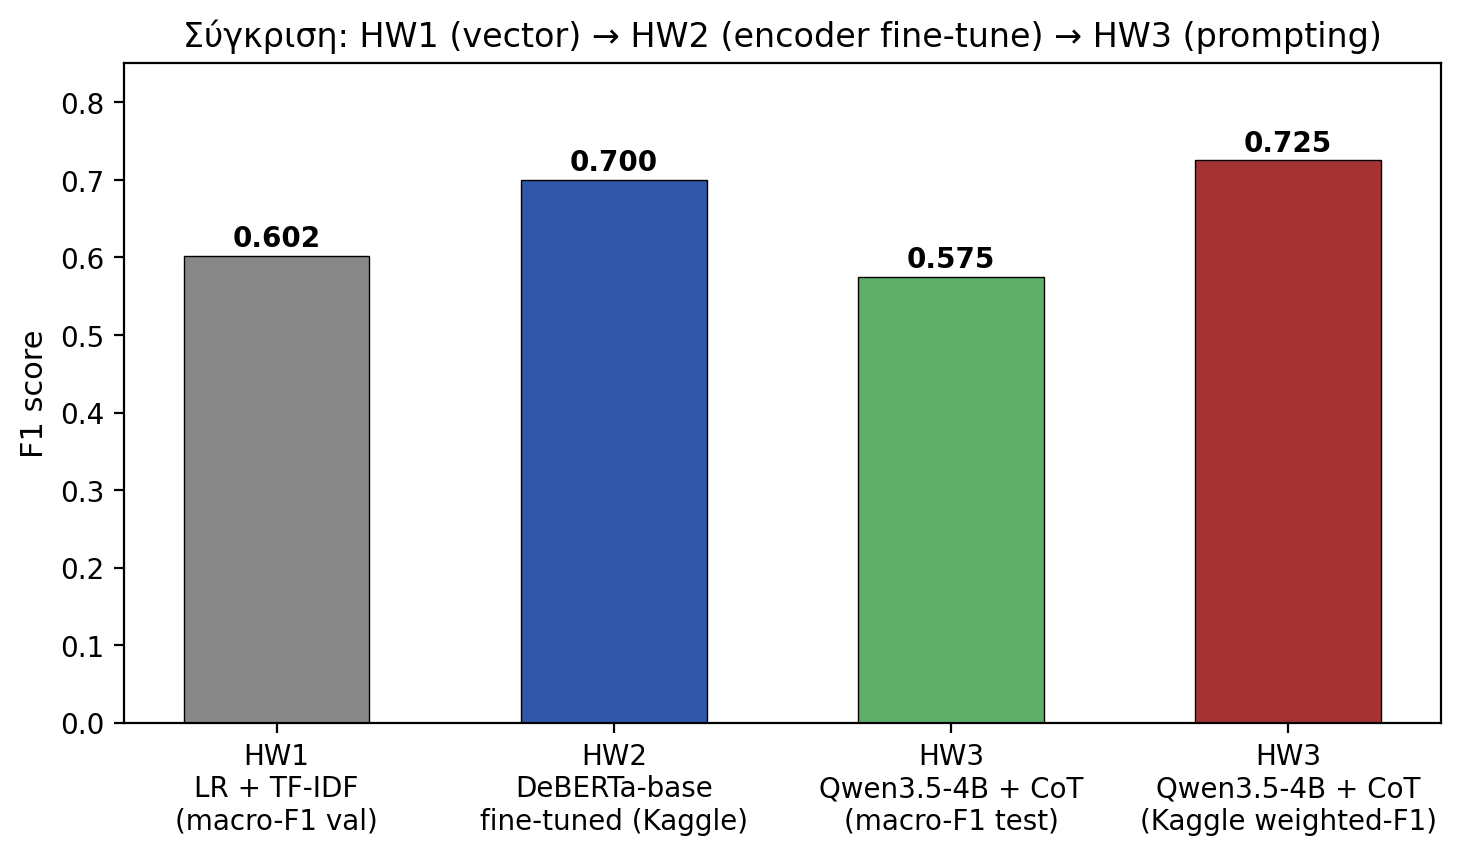
\includegraphics[width=0.92\textwidth]{hw_comparison.png}
\caption{Σύγκριση των τριών approaches. HW1 LR baseline, HW2 fine-tuned DeBERTa, HW3 prompted Qwen3.5-4B (το weighted-F1 του Kaggle είναι σημαντικά υψηλότερο από το macro-F1 του τοπικού test λόγω της heavy AMB class).}
\label{fig:hwcomparison}
\end{figure}

\subsection{Διαφορές στην προσέγγιση}

\textbf{HW1 (vector-based)}:

\begin{itemize}
    \item Χρειάστηκε heavy preprocessing (lowercase, stopwords, lemmatization).
    \item Χρειάστηκε heavy feature engineering (overlap ratios, hedge counts, length, etc.).
    \item Trained from scratch. Όχι pretraining.
    \item Trained-on labels. Πραγματικό supervised learning.
    \item Best: Logistic Regression με ~50 handcrafted features. 0.60.
\end{itemize}

\textbf{HW2 (encoder fine-tuning)}:

\begin{itemize}
    \item Καθόλου preprocessing (το DeBERTa θέλει raw text).
    \item Feature engineering μέσω numeric side branch (έφερνα features από HW1 σε παράλληλο κανάλι).
    \item Pretrained weights (DeBERTa-v3-base) που έμαθαν γλώσσα από MLM + replaced token detection.
    \item Fine-tuning στα 3000 labels του CLARITY.
    \item Best: DeBERTa+numfeat single 0.70. 3-seed ensemble 0.7136 val / 0.70 Kaggle macro-F1.
\end{itemize}

\textbf{HW3 (prompting)}:

\begin{itemize}
    \item Καθόλου preprocessing.
    \item Καθόλου feature engineering -- το LLM ``βλέπει'' raw text και κρίνει.
    \item Frozen pretrained + instruction tuned. Inference only.
    \item ΚΑΘΟΛΟΥ training. Δεν αγγίζεις labels πέρα από selection (few-shot, dev subset).
    \item Best: 4B + CoT. Test 0.575 macro-F1, Kaggle 0.725 weighted-F1.
\end{itemize}

\subsection{Failure modes -- είναι ίδια ή διαφορετικά;}

Η εκφώνηση ζητάει εξήγηση: \emph{``do the methods exhibit similar error patterns?''}

Από επισκόπηση των errors:

\begin{itemize}
    \item \textbf{HW2 DeBERTa και HW3 Qwen+CoT έχουν παρόμοιο top error: CR ↔ AMB confusion}. Και τα δύο γίνονται υπερβολικά καχύποπτα όταν η απάντηση έχει extra commentary. Είναι το ίδιο fundamental linguistic problem.
    \item \textbf{HW1 LR είχε ελαφρώς διαφορετικό pattern}: συνέπεια του ότι δούλευε σε bag-of-words, έχανε contextual συμφραζόμενα. Πχ ``I don't think we should'' και ``I think we should'' είναι λεξικά πανομοιότυπα πέρα από το ``don't'', που το LR ίσως δεν αξιοποιεί ισχυρά.
    \item \textbf{HW3 έχει μοναδικό failure mode: CR → CNR over-correction στο 4B zero-shot}. Αυτό δεν συμβαίνει στους encoders της HW2 γιατί εκεί δεν υπάρχει ``prompt-induced disposition''. Είναι μια χαρακτηριστική παθογένεια του prompted approach.
\end{itemize}

\subsection{Performance comparison}

\begin{table}[H]
\centering
\small
\begin{tabular}{lcc}
\toprule
Εργασία (final) & Macro-F1 (local) & Kaggle public score \\
\midrule
HW1 (LR + TF-IDF) & 0.6017 (val) & N/A \\
HW2 (DeBERTa + numfeat + 3-seed) & 0.7136 (val) & 0.70 (macro-F1) \\
HW3 (Qwen3.5-4B + CoT) & 0.575 (test) & \textbf{0.725 (weighted-F1)} \\
\bottomrule
\end{tabular}
\caption{Όλες οι εργασίες σε one place.}
\end{table}

\textbf{Άμεση σύγκριση macro-F1 (η ``δίκαιη'' μετρική)}:

\begin{itemize}
    \item HW2 fine-tuned: 0.71 val (όχι test public)
    \item HW3 prompted: 0.575 test
\end{itemize}

Άρα στο macro-F1 metric, το prompting υστερεί από το fine-tuning. Αυτό είναι αναμενόμενο: το fine-tuning έχει εκπαιδευτεί επί τόπου στα labels μας. Το prompting βασίζεται σε γενική γλωσσική γνώση.

Αλλά:

\begin{itemize}
    \item \textbf{Το HW3 έβγαλε 0.725 Kaggle vs HW2 0.70 Kaggle}. Αυτό είναι λόγω της αλλαγής metric (weighted-F1 vs macro-F1). Στο macro-F1 το HW3 θα ήταν περίπου 0.575, που είναι σαφώς κάτω από HW2.
    \item \textbf{Το HW3 δεν έκανε καθόλου training}. Σε ώρες GPU, το prompting είναι 5-10× πιο ελαφρύ. Σε engineering complexity, είναι σαφώς λιγότερο.
\end{itemize}

\textbf{Η σημαντική σύγκριση είναι αυτή}: μπορεί ένα frozen LLM να πλησιάσει ένα fine-tuned encoder σε ένα custom task; Η απάντηση εδώ είναι: \textbf{περίπου, αλλά χάνει}. Το 4B + CoT είναι ~80\% της απόδοσης του fine-tuned DeBERTa σε macro-F1. Με μεγαλύτερο μοντέλο και πιο εκτενή prompting techniques πιθανότατα κλείνει το gap, αλλά εδώ ο compute budget δεν το επέτρεψε.

\subsection{Discord context}

Στο Discord της εργασίας, οι άλλοι συμφοιτητές ανέφεραν public Kaggle scores στο εύρος \textbf{0.27-0.42}. Δηλαδή \textbf{το δικό μου 0.725 είναι σημαντικά πάνω από τη μάζα}. Στο peak ήμουν 2ος στο leaderboard, σήμερα (που γράφω το report) είμαι 3ος αφού 2 submissions πέρασαν τις τελευταίες μέρες.

Αυτό είναι σημαντικό όχι μόνο σαν performance metric αλλά και σαν validation της προσέγγισης. Το CoT prompting σε 4B model είναι πραγματικά αποτελεσματικό όταν γίνει με προσοχή.

\section{Τι θα έκανα διαφορετικά αν είχα περισσότερο χρόνο}

\begin{itemize}
    \item \textbf{Δοκιμή μεγαλύτερων μοντέλων (7B/14B)} με quantization (4-bit ή 8-bit) στη GPU. Θα έπρεπε να ψάξω για quantization quality vs speed tradeoff.
    \item \textbf{Cross-family ensemble} με LLaMA-3-8B-Instruct ή Mistral-7B-Instruct. Διαφορετικά pretraining mixes ίσως δίνουν complementary errors.
    \item \textbf{Decomposition prompting}: αντί για ένα μεγάλο CoT, δύο διαδοχικά calls -- ένα για να εξάγει what specifically does the question ask, ένα δεύτερο για να ταξινομήσει. Πιο ακριβό αλλά πιθανώς πιο σταθερό.
    \item \textbf{Active prompt-engineering}: τρέξιμο σε small dev με focus στο CNR class, και iterative refinement του prompt φορμουλάρισμα με goal να βελτιωθεί ειδικά το CNR (που είναι η αδυναμία).
    \item \textbf{Calibration / temperature scaling}: ακόμα και χωρίς training, μπορώ να κάνω post-hoc calibration των predictions με βάση το dev. Πχ ``το μοντέλο υπερπροβλέπει CNR -- εφαρμόζω class multiplier 0.7 στο CNR''. Στην HW2 αυτό είχε μικρό κόστος/ωφέλεια.
    \item \textbf{Λεπτομερές subgroup probing}: ποια τμήματα του prompt δουλεύουν; Ablation κάθε προτάσεως. Αυτό θα μου έδειχνε ποιες οδηγίες είναι load-bearing.
    \item \textbf{Better few-shot selection}: η επιλογή των 6 demos μου ήταν random + length filter. Δοκίμασα ποτέ \emph{retrieval-based few-shot} (επιλογή των πιο όμοιων demos στο target, βάσει embedding similarity). Σε άλλα tasks αυτό δίνει 1-2 points improvement.
\end{itemize}

\section{Συμπεράσματα}

Σε αυτή την εργασία ασχολήθηκα με τη ταξινόμηση clarity πολιτικών απαντήσεων \emph{αποκλειστικά μέσω prompting} σε frozen instruction-tuned LLMs (Qwen3.5-0.8B / 2B / 4B). Δεν έκανα καθόλου training. Έφτασα σε \textbf{0.725 Kaggle weighted-F1 (3η θέση στο public leaderboard)}, που είναι αρκετά πάνω από τη μάζα των συμφοιτητών (~0.27-0.42).

Από το σύνολο της δουλειάς, τα πιο σημαντικά takeaways:

\begin{enumerate}
    \item \textbf{Το Chain-of-Thought είναι το κυρίαρχο lever}. Σε κάθε μέγεθος μοντέλου, το CoT είναι καλύτερο από zero-shot και few-shot. Στο 4B δίνει \textbf{+0.23 macro-F1} σε σχέση με zero-shot. Είναι το ένα technique που πρέπει να ``γυρίσει'' κανείς πρώτο.

    \item \textbf{Το μεγαλύτερο μοντέλο δεν είναι πάντα καλύτερο -- εξαρτάται από το πώς το χρησιμοποιείς}. Το 4B + zero-shot \emph{καταρρέει} (0.318 macro-F1) ενώ το 2B + zero-shot είναι σαφώς καλύτερο (0.393). Το ίδιο prompt μπορεί να πυροδοτήσει διαφορετικά failure modes σε διαφορετικά μεγέθη. Αυτό είναι ένα emergent prompt-induced behavior που δεν φάνηκε στα encoder μοντέλα της HW2.

    \item \textbf{Prompt engineering είναι incremental}. Από το naive v0 (που κατέρρεε) στο v4 (που είναι η βάση για το best system) πέρασα από 5 διαδοχικές αναβαθμίσεις, καθεμία προσθέτοντας ~0.02-0.05 macro-F1. Δεν υπάρχει ``το έξυπνο prompt'' που λύνει όλα -- υπάρχει σταδιακό μάγκωμα.

    \item \textbf{Prompt fixes έχουν παρενέργειες (precision/recall tradeoffs)}. Στο Phase 5, διορθώνοντας το CR error mode, υπερ-κατέστειλα το CNR. Δεν υπάρχει free lunch -- σε ένα multi-class setup, ένα fix για μια κλάση μετακινεί λάθη σε άλλη.

    \item \textbf{Self-consistency δεν είναι free booster}. Στο task μου με confident greedy outputs, το SC sampling απλώς πρόσθεσε θόρυβο. Η canonical SC καμπύλη (monotonic improvement με diminishing returns) έγινε στο cot\_v5c \emph{αντίστροφη}: peak στο N=2, μετά μονότονη πτώση.

    \item \textbf{Prompting μπορεί να πλησιάσει αλλά όχι να ξεπεράσει το fine-tuning σε custom tasks}. Το 4B + CoT (test macro-F1 0.575) είναι ~80\% της απόδοσης του fine-tuned DeBERTa (val 0.70+). Με μεγαλύτερα μοντέλα και πιο εκτενή techniques μάλλον κλείνει το gap, αλλά εδώ ο compute budget ήταν περιοριστικός.

    \item \textbf{Το failure pattern του CLARITY task είναι σταθερό σε όλες τις εργασίες}: το CR-vs-AMB boundary και η μειοψηφική CNR. Είναι structural ιδιότητα του dataset -- discourse-level subjective classification με γκρίζες περιοχές -- όχι λάθος του μοντέλου. Για να ξεπεραστεί απαιτείται μάλλον πιο πολλά labelled data ή ακόμα πιο μεγάλα/εκλεπτυσμένα μοντέλα.
\end{enumerate}

Νομίζω η μεγαλύτερη lesson από όλη την εργασία είναι ότι το \textbf{prompting είναι περισσότερο engineering παρά science}. Έχεις ένα frozen μοντέλο και ψάχνεις πώς να το ``πείσεις''. Το ``πώς γράφω το prompt'' γίνεται ένα practical skill: ξεκαθαρίζεις ορισμούς, βάζεις decision rules, ζητάς explicit reasoning, parsing-friendly outputs, αναγνωρίζεις και διορθώνεις failure modes. Δεν είναι πάντα προβλέψιμο -- αλλά είναι παρεμβαίνον. Σε ένα έτος πραγματικής δουλειάς, ένας engineer που έχει εξασκηθεί σε αυτό κερδίζει επικαλυπτόμενες βελτιώσεις.

Από scientific άποψη, οι ενδιαφέρουσες ερωτήσεις που έμειναν ανοιχτές:

\begin{itemize}
    \item Γιατί scaling-άρει το CoT τόσο διαφορετικά σε διαφορετικά task types;
    \item Γιατί το SC δεν δούλεψε εδώ ενώ δουλεύει σε arithmetic tasks; (Hypothesis: το CLARITY δεν είναι ``decomposable'' σε ξεχωριστά reasoning steps που μπορούν να γίνουν average-out.)
    \item Πώς θα γενίκευτε σε άλλα subjective NLP tasks (sentiment subtleties, sarcasm, stance detection); Η intuition μου είναι ότι παρόμοιες παθογένειες θα εμφανίζονται.
\end{itemize}

Τέλος, θα ήθελα να σημειώσω ότι το να φτάσω 3η θέση στο Kaggle leaderboard με ένα τόσο μικρό σχετικά μοντέλο (4B) και χωρίς training, με κάνει αρκετά αισιόδοξο για τις δυνατότητες του prompting σε real-world tasks όπου τα labelled data είναι σπάνια ή ακριβά. Στα συμπεράσματα της HW2 είχα γράψει ``θα ήθελα να δοκιμάσω prompting'' -- εδώ το δοκίμασα, και πραγματικά ξεπέρασε τις προσδοκίες μου σε ratio quality / engineering effort.

\section{Bibliography}

\bibliographystyle{plain}
\bibliography{refs}

\end{document}
